%%%%%%%%%%%%%%%%%%%%%%%%%%%%%%%%%%%%%%%%%%%%%%%%%%%%%%%%%%%%%%%%%%%%%%%%%%%%%%%%%%%%%%%%%%
\section{Results}

%%%%%%%%%%%%%%%%%%%%%%%%%%%%%%%%%%%%%%%%%%%%%
\subsection{Franke Data}
\begin{figure}[H]
    \centering
    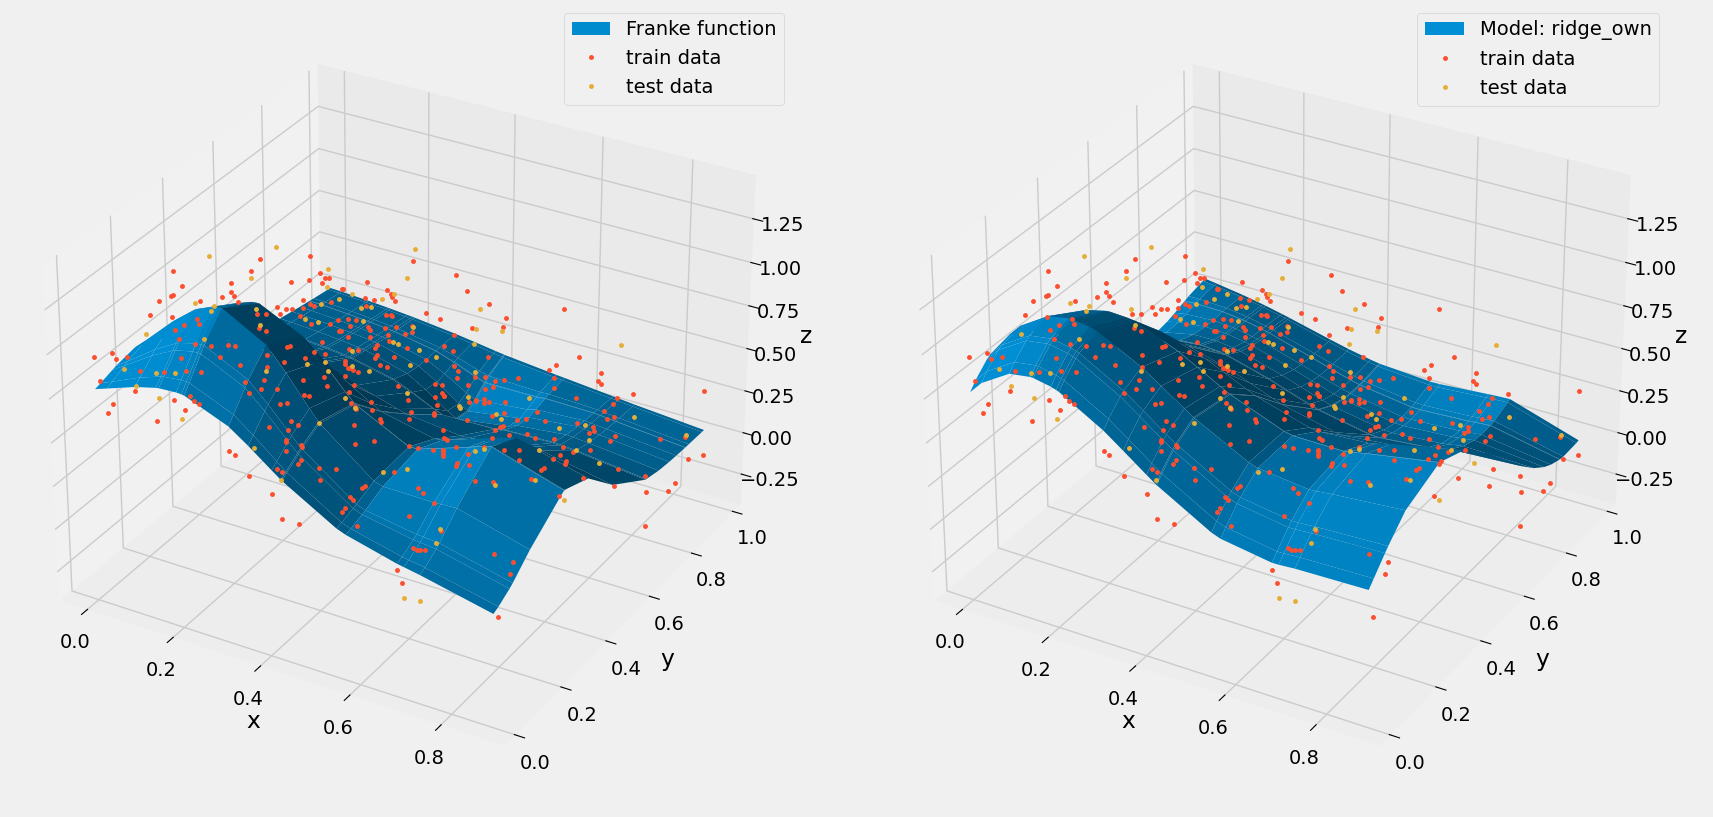
\includegraphics[width=0.8\textwidth]{Figures/franke_data_and_model_ridge_best.png}
    \caption{Left figures shows the frank function plotted as a function of x
    and in y coordinates the intervall [0,1]. The red and yellow dots shows or
train- and test-data with added normal distributed noise, $0.2 \cdot
\sigma(0,1)$. The lowest MSE, calculated with bootstrap re-sampling was obtained
with Ridge regression with a regularization parameter $\lambda = 10^{-5}$ and a
polynomial degree of 5. Right figure shows the best fit model. Train- and
test-data is plotted as for the left figure.} 
\end{figure}

\begin{figure}
     \centering
     \begin{subfigure}[t]{0.49\textwidth}
         \centering
         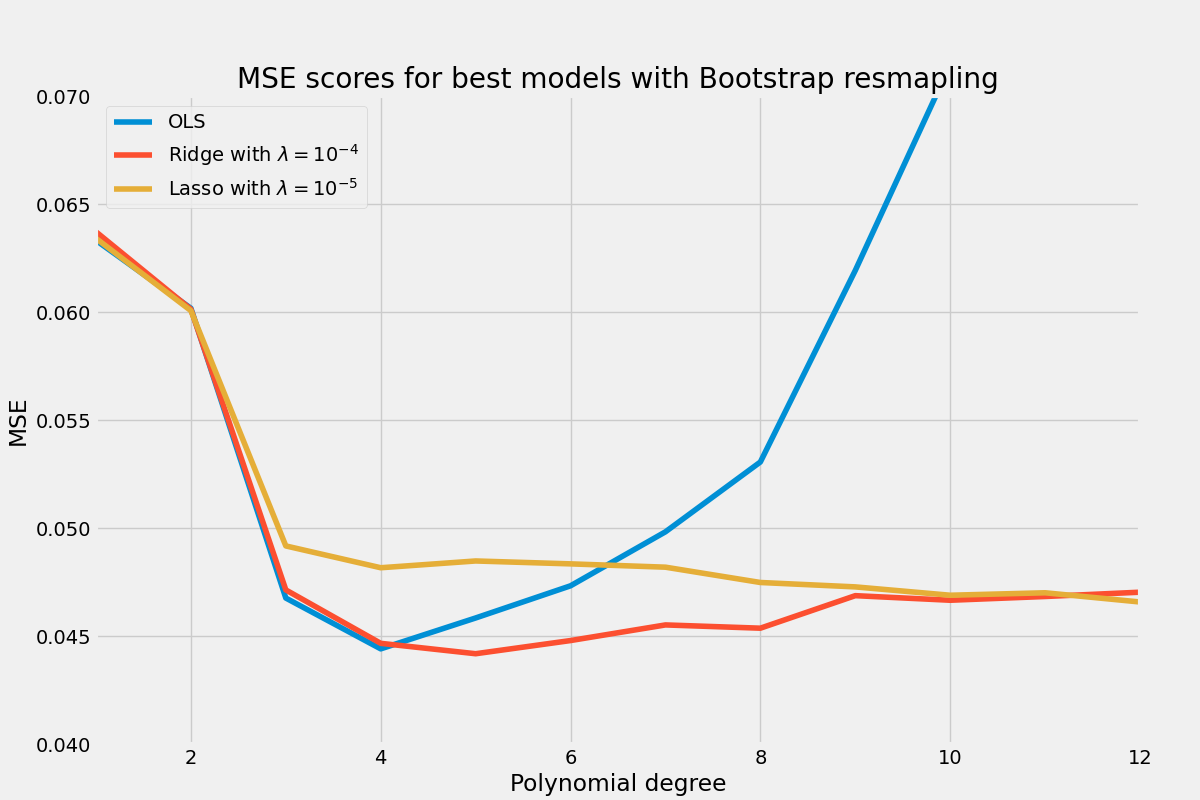
\includegraphics[width=\textwidth]{Figures/franke_ols_ridge_lasso_boots.png}
         \caption{Mean MSE score for 100 bootstrap re-samples. MSE scores is
             plotted as a function of polynomial degree, for the best fit
             models obtained with OLS, Ridge ($\lambda =
             10^{-j}$) and Lasso ($\lambda = 10^{-5}$) regression.}  
         \label{} 
     \end{subfigure}
     \hfill
     \begin{subfigure}[t]{0.49\textwidth}
         \centering
         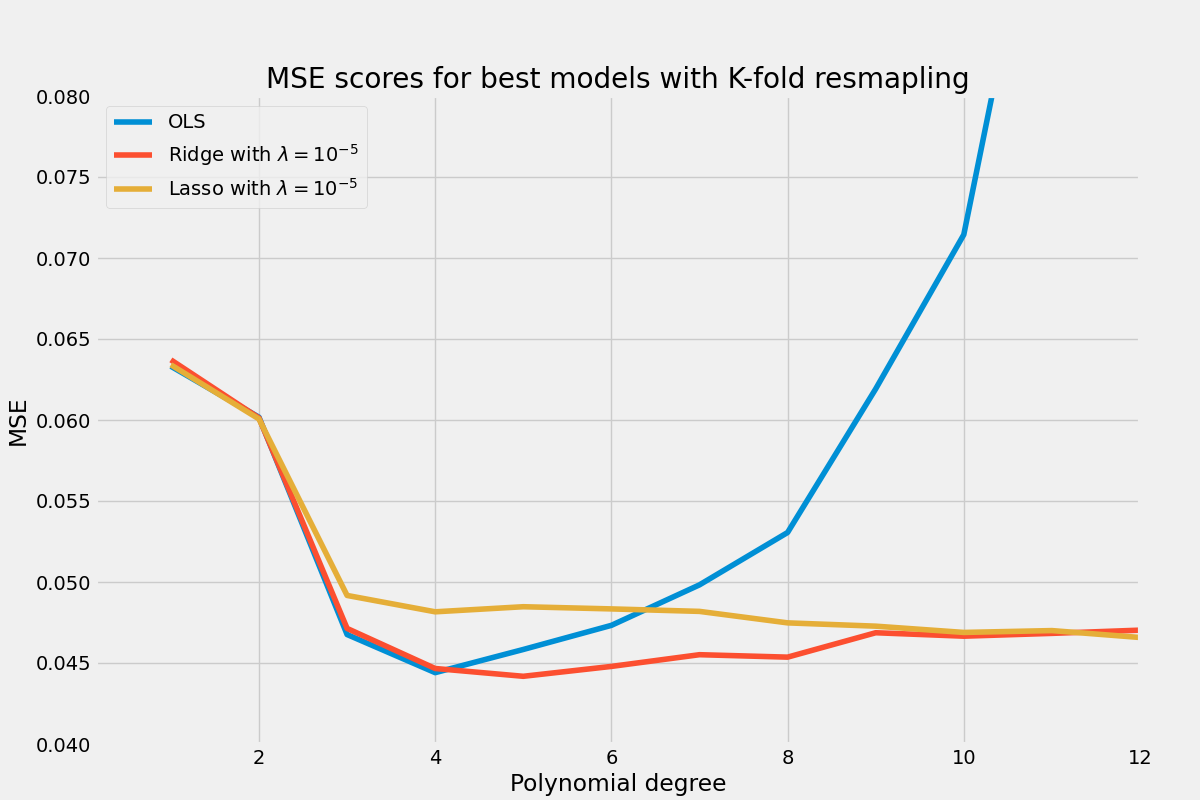
\includegraphics[width=\textwidth]{Figures/franke_ols_ridge_lasso_kfold.png}
         \caption{Mean of MSE scores calculated on all ten test folds with K-fold
             re-sampling. Our best fit models from OLS, Ridge ($\lambda =
             10^{5}$) and Lasso ($10^{-5}$) regression
     is plotted as a function of polynomial degree. $\lambda $ is the 
 regularization parameter.}  
         \label{fig}
     \end{subfigure}

\end{figure}


\begin{table}
    \centering
    \caption{Table of Best mean squared error (MSE) scores obtained with
        different re-sampling and regression
        methods. The training- and testing-data splits from the Franke function
        was used for model fitting and
        prediction respectively. $\lambda $ is the best choice of regularization parameters for
        Ridge and Lasso regression. n refers to number of re-samples/splits used in
        Bootstrap and K-fold.}  
    \label{tab:franke_mse_best} 
    \begin{tabular}{|c|c|c|c|c|}
        \hline
        Polynomial degree & $\lambda$ & Regression method & Re-sampling method & MSE \\
        \hline
                      4    &    & OLS & Bootstrap (n=100) & 0.04440 \\
        \hline
                      5   & $10^{-4}$  & Ridge & Bootstrap (n=100)& 0.04425 \\
        \hline
                      11  & $10^{-5}$  & Lasso & Bootstrap (n=100)& 0.04673 \\
                      
        \hline
                      5    &   & OLS &  K-fold (n=10) &  0.04181\\
        \hline
                      6   &  $10^{-5}$  & Ridge &  K-fold (n=10) & 0.04155 \\
        \hline
                      12  &  $10^{-5}$ & Lasso &  K-fold (n=10) & 0.04548 \\
        \hline
    \end{tabular} 
\end{table}

% TODO OLS scores

%%%%%%%%%%%%%%% Parameters %%%%%%%%%%%%%%%
% n_data = 20 - n_data in x and y: n_tot = 20*20
% test_size = 0.2
% noise = 0.2 - aptitude of normal distributed noise    
% data_dim = 2

%%%%%%%%%%%%%%% Part b %%%%%%%%%%%%%%%
% * Evaluate MSE up to 5.th order fro OLS. 
% * and R2 score
% * blot parameters beta
% * Your code has to include a scaling/centering:
%   XXX: not included, data is already scaled in intervall [-1, 1]

\begin{figure}
     \centering
     \begin{subfigure}[b]{0.5\textwidth}
         \centering
         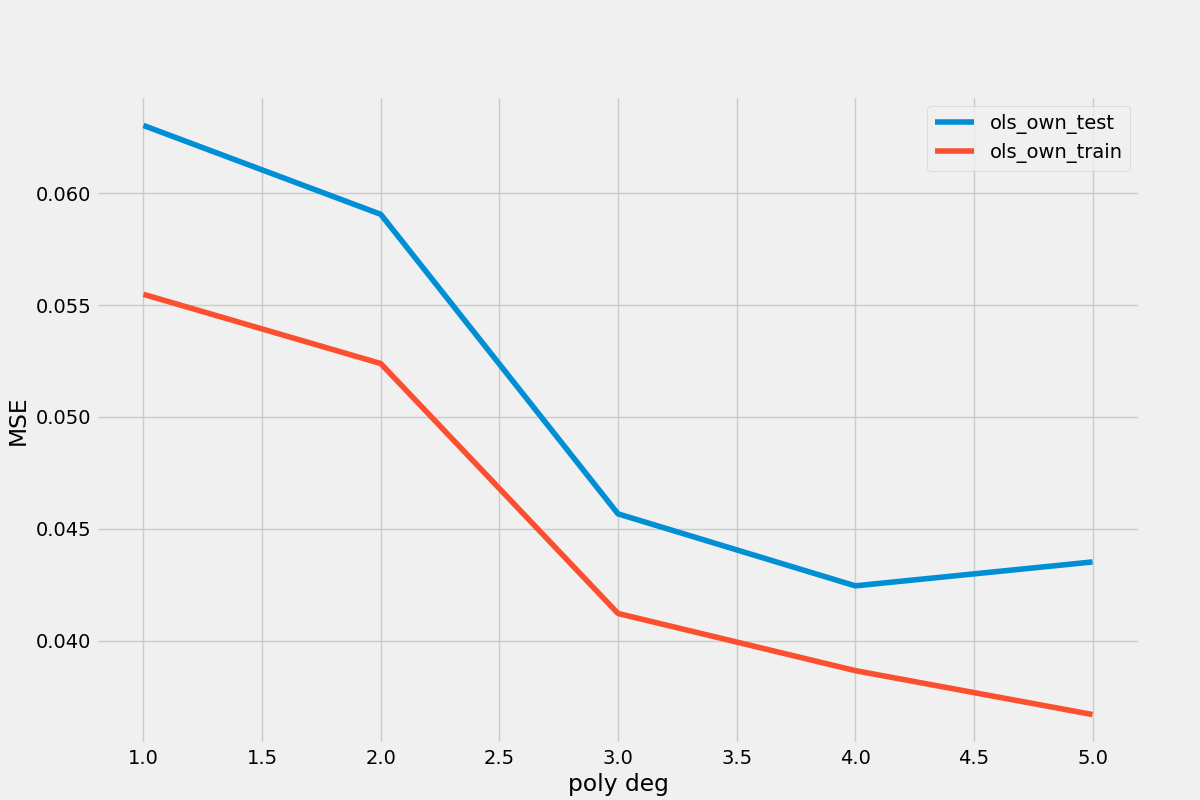
\includegraphics[width=\textwidth]{Figures/b_mse.png}
     \end{subfigure}%
     \hfill
     \begin{subfigure}[b]{0.5\textwidth}
         \centering
         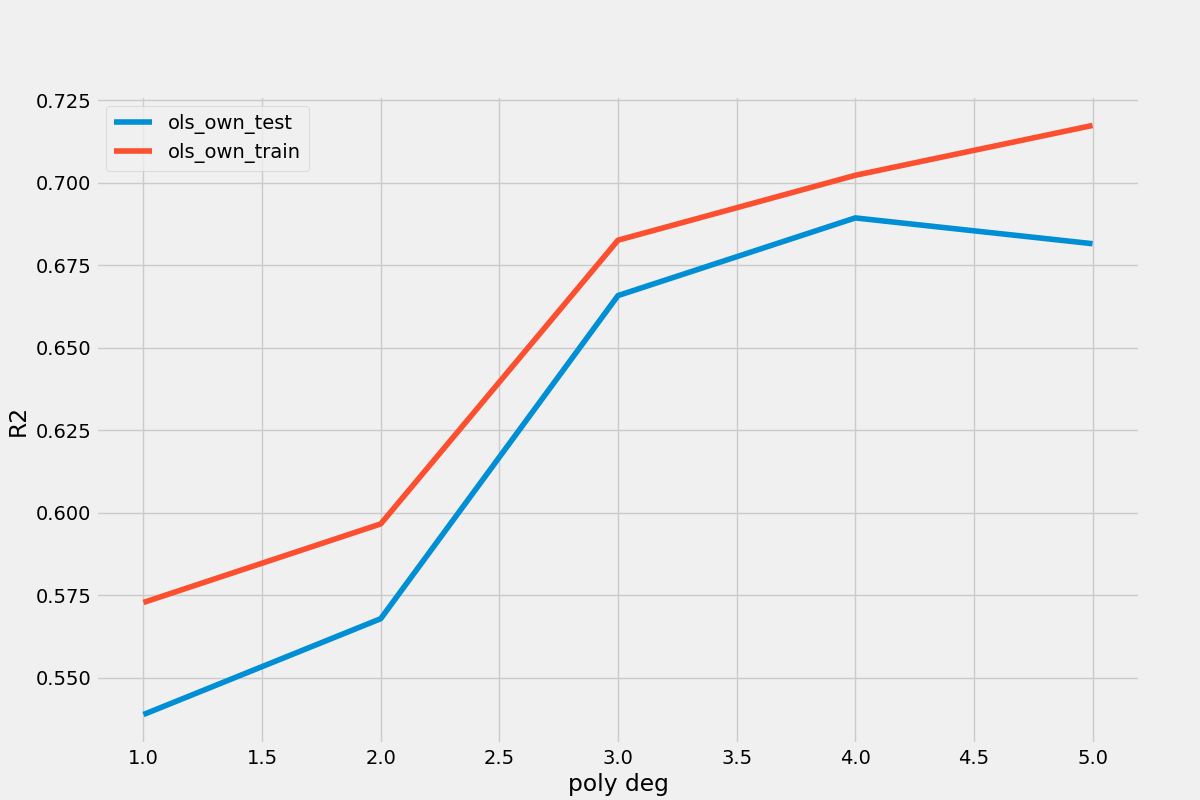
\includegraphics[width=\textwidth]{Figures/b_r2.png}
     \end{subfigure}
        \caption{Mean squared error and score function for the Ordinary Least Squares (OLS) method on the Franke function with N=????? for training and test data with a test/train split of 0.2}
        \label{fig:mse_and_score_franke}
\end{figure}

In figure \ref{fig:mse_and_score_franke} we see the mean squared error and score on the Franke function for a polynomial up to degree five. If our predictors represent different scales, then it is important to standardize the design matrix. And as the x and y data is on the same interval $[0, 1]$ we do not need to scale the data. We see from the figure that we get a big decrease in MSE and big increase in $R^2$ for a polynomial degree up to five. For degree five we do not see much change. 

%\begin{figure}[H]
%    \centering
%    \caption{Mean square error as function of polynomial degree for }
%    \label{fig:ols_franke}
%    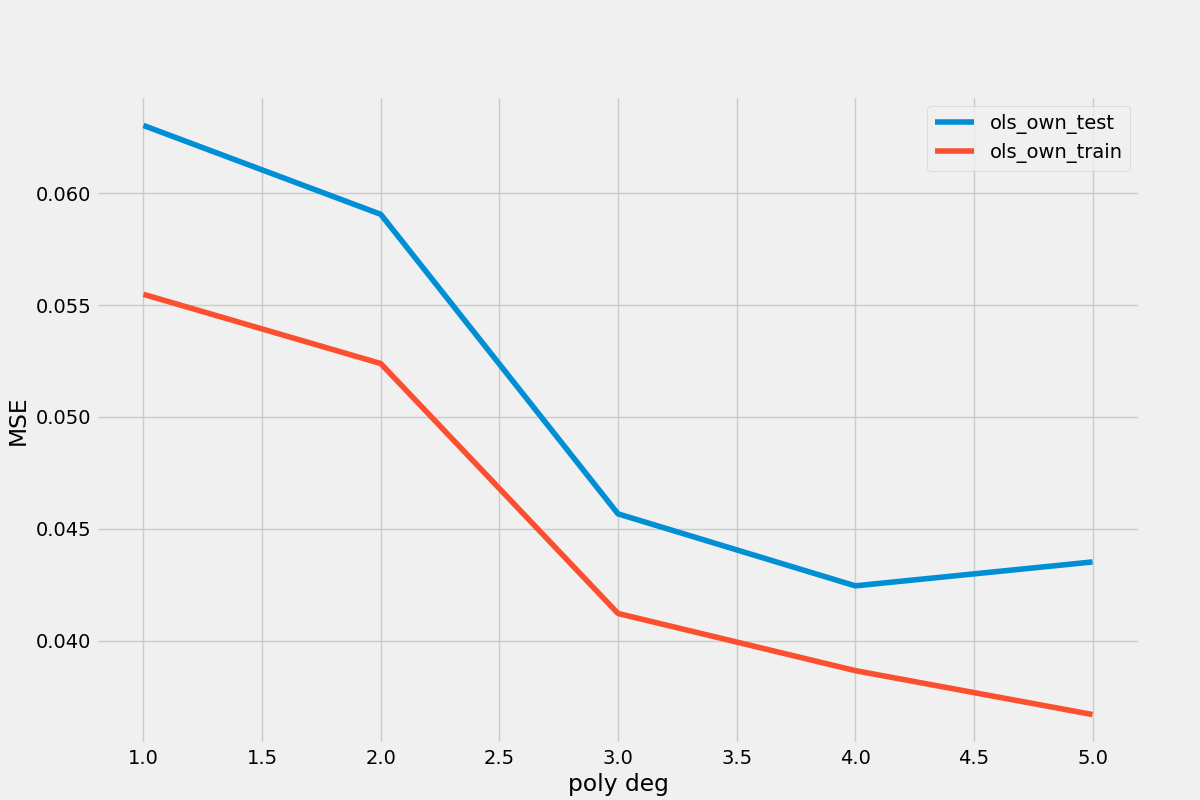
\includegraphics[width=0.8\textwidth]{Figures/b_mse.png}
%\end{figure}

%\begin{figure}[H]
%    \centering
%    \caption{}
%    \label{fig:score_franke}
%    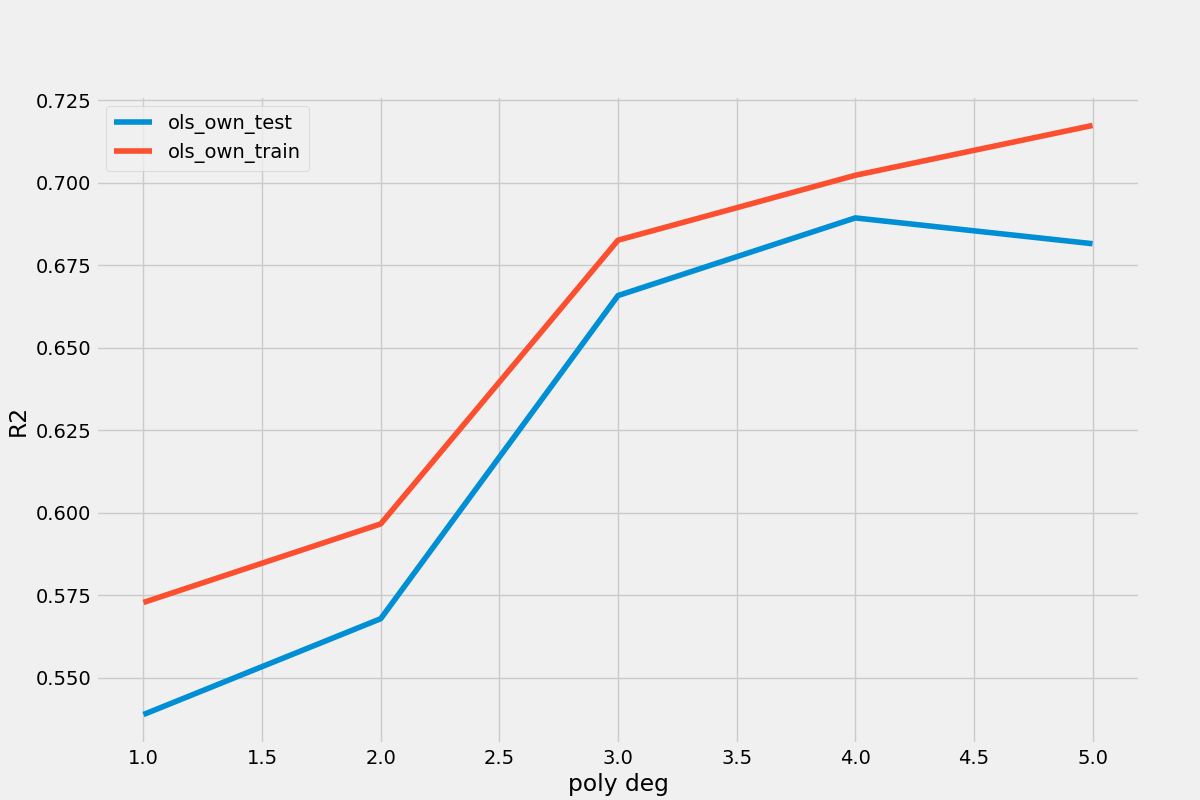
\includegraphics[width=0.8\textwidth]{Figures/b_r2.png}
%\end{figure}

% TODO: error bars
\begin{figure}[H]
    \centering
    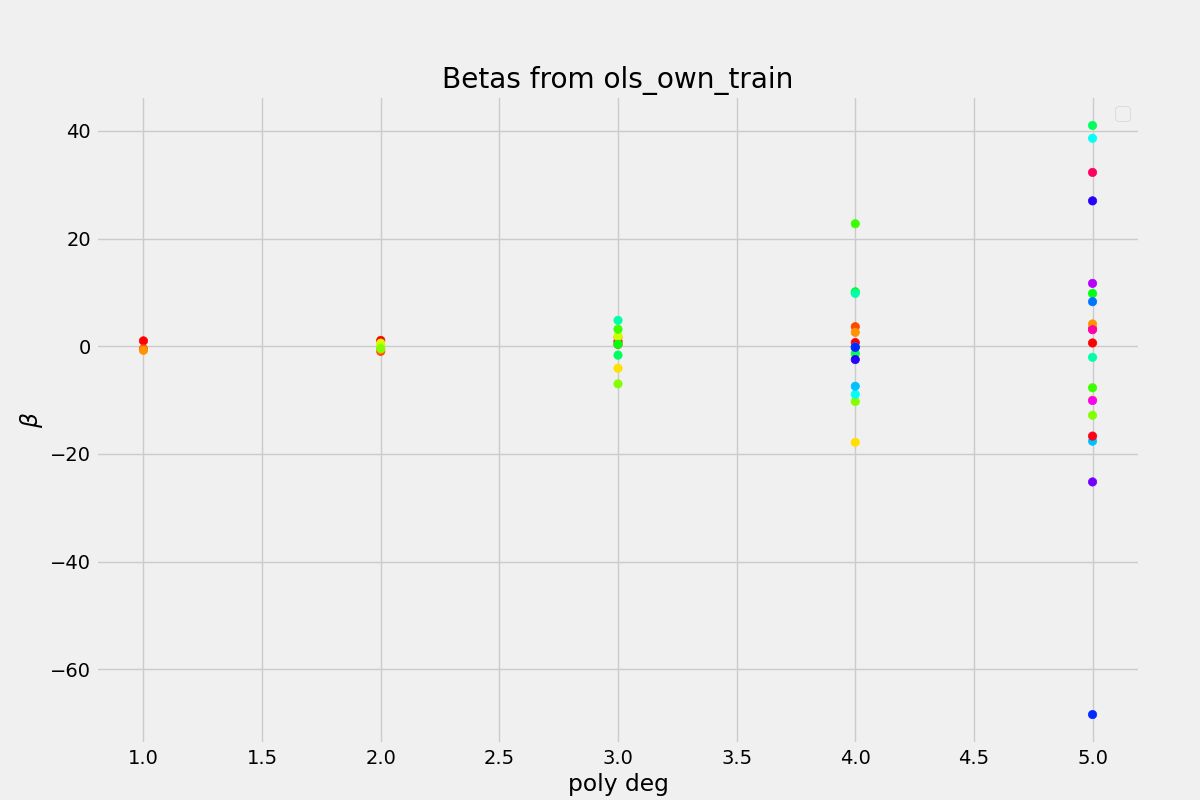
\includegraphics[width=0.8\textwidth]{Figures/b_beta.png}
    \label{fig:beta_plot}
    \caption{$\beta$-parameters of the OLS model on the Franke function for N=????. Ment to illustrate variation in $\beta_i$ as polynomial degree increases.}
\end{figure}

In figure \ref{fig:beta_plot} we see for each polynomial degree the beta parameters $\beta_i$ as a dot in the plot. This is for the OLS model on the Franke function. We see that as the polynomial degree increases, the $\beta$ values deviate more and more from zero. This can be a result of overfitting since we do not have any regularization parameter on the OLS model.

%For bootstrap: should consider plotting a histogram of the estimators beta_hat^* as this should resemble a pdf. 

%%%%%%%%%%%%%%% Part c  %%%%%%%%%%%%%%%
% * Explain bias, variance, mse terms (theory) and interpretation 
% * Bias variance analysis on franke function
% * discuss in bias variance trade-off in terms of:
%   * model complexity
%   * number of data points
%   * training and test data

%%bootstrap figures for different number of datapoints
\begin{figure}
     \centering
     \begin{subfigure}[b]{0.5\textwidth}
         \centering
         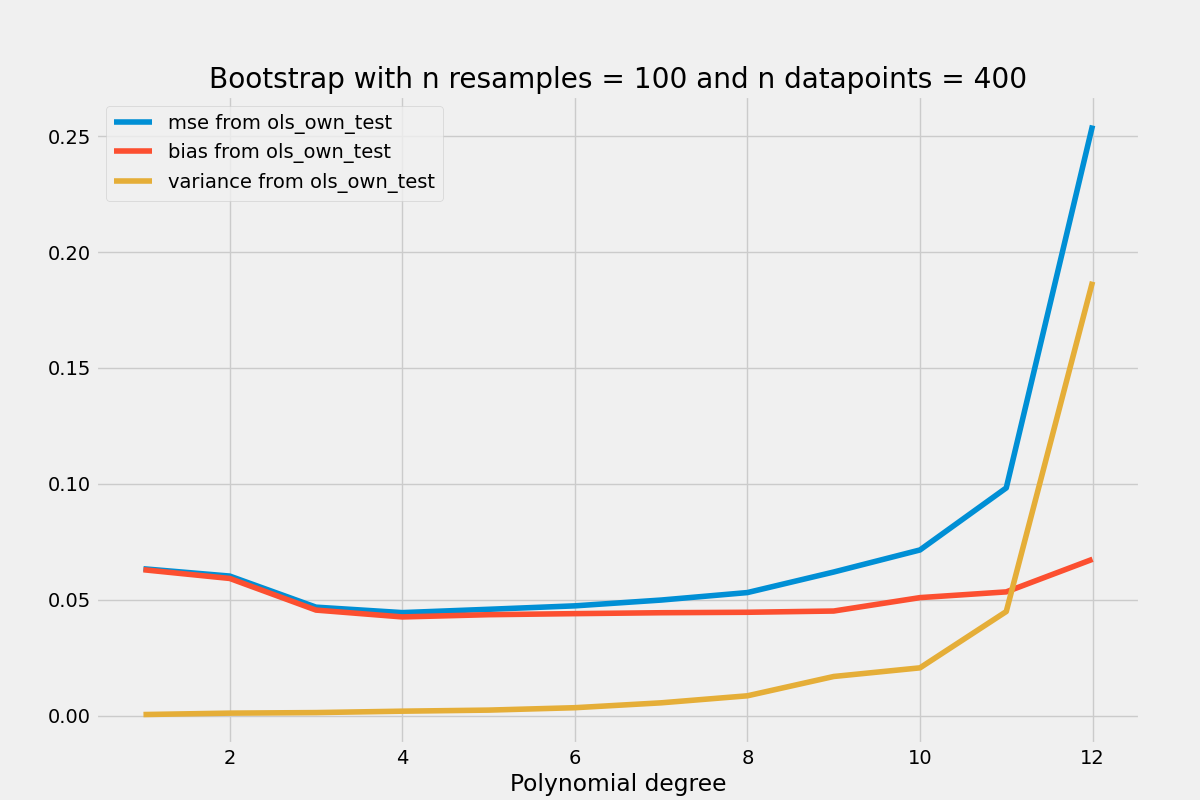
\includegraphics[width=\textwidth]{Figures/c_bootstrap_ols_n_data_400.png}
         \caption{400 datapoints}
     \end{subfigure}%
     \hfill
     \begin{subfigure}[b]{0.5\textwidth}
         \centering
         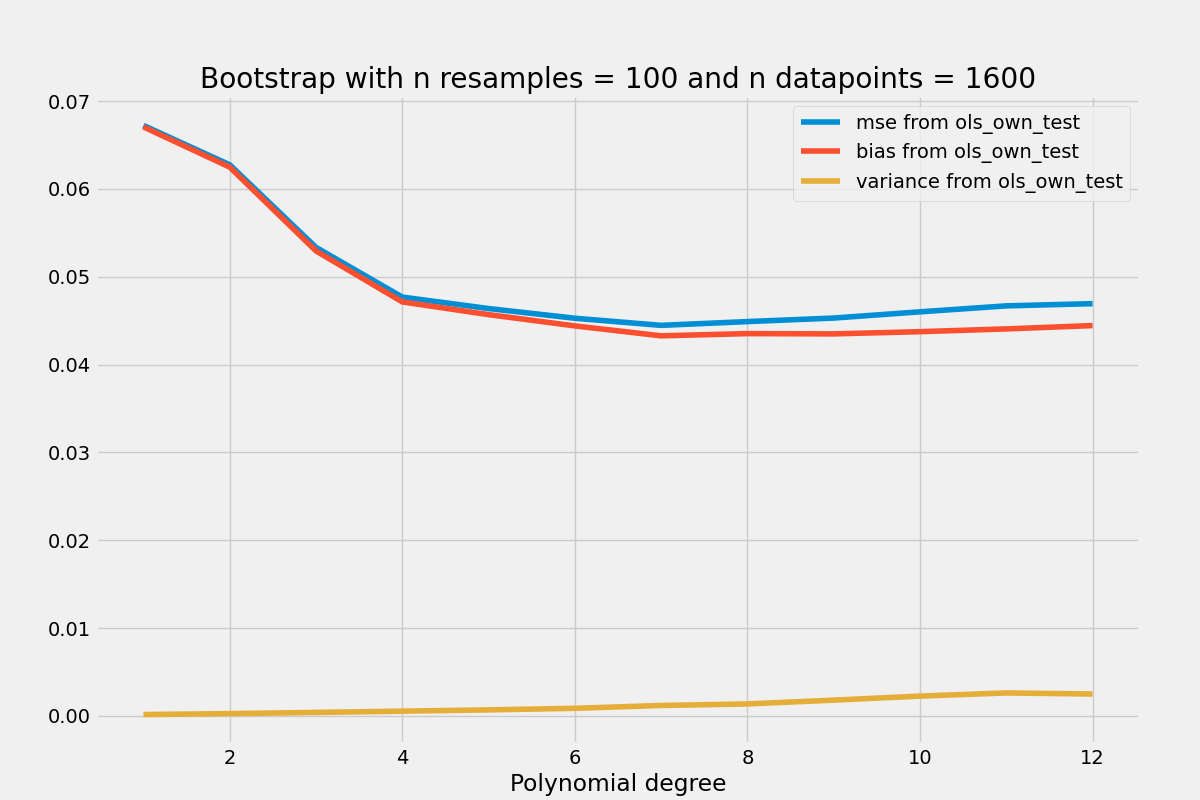
\includegraphics[width=\textwidth]{Figures/c_bootstrap_ols_n_data_1600.png}
         \caption{1600 datapoints}
     \end{subfigure}
        \caption{Bootstrap with 100 resamples for the OLS method on the Franke function on the test set.}
        \label{fig:bootstrap_ols_franke_test}
\end{figure}

In figure \ref{fig:bootstrap_ols_franke_test} we can see the the bootstrap used on the OLS method on the Franke function for 100 resamples and two different number of datapoints. We see that for the lower number of points we get signs of overfitting, while we do not see this behaviour at these polynomial degrees for 1600 datapoints. We see that for 400 datapoints the optimal bias-variance tradeoff happens at a polynomial degree of around 4 and for 1600 datapoints at around polynomial degree 7.


%\begin{figure}[H]
%    \centering
%    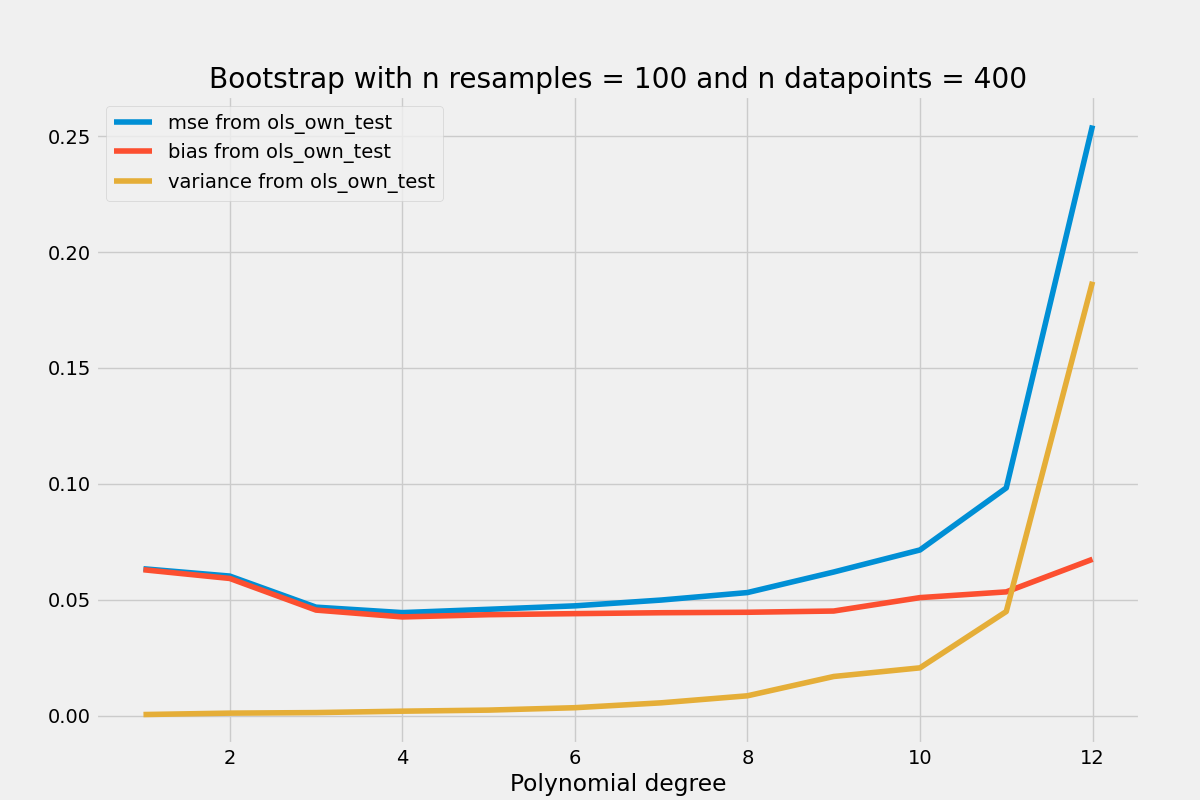
\includegraphics[width=0.8\textwidth]{Figures/c_bootstrap_ols_n_data_400.png}
    
%\end{figure}


%\begin{figure}[H]
%    \centering
%    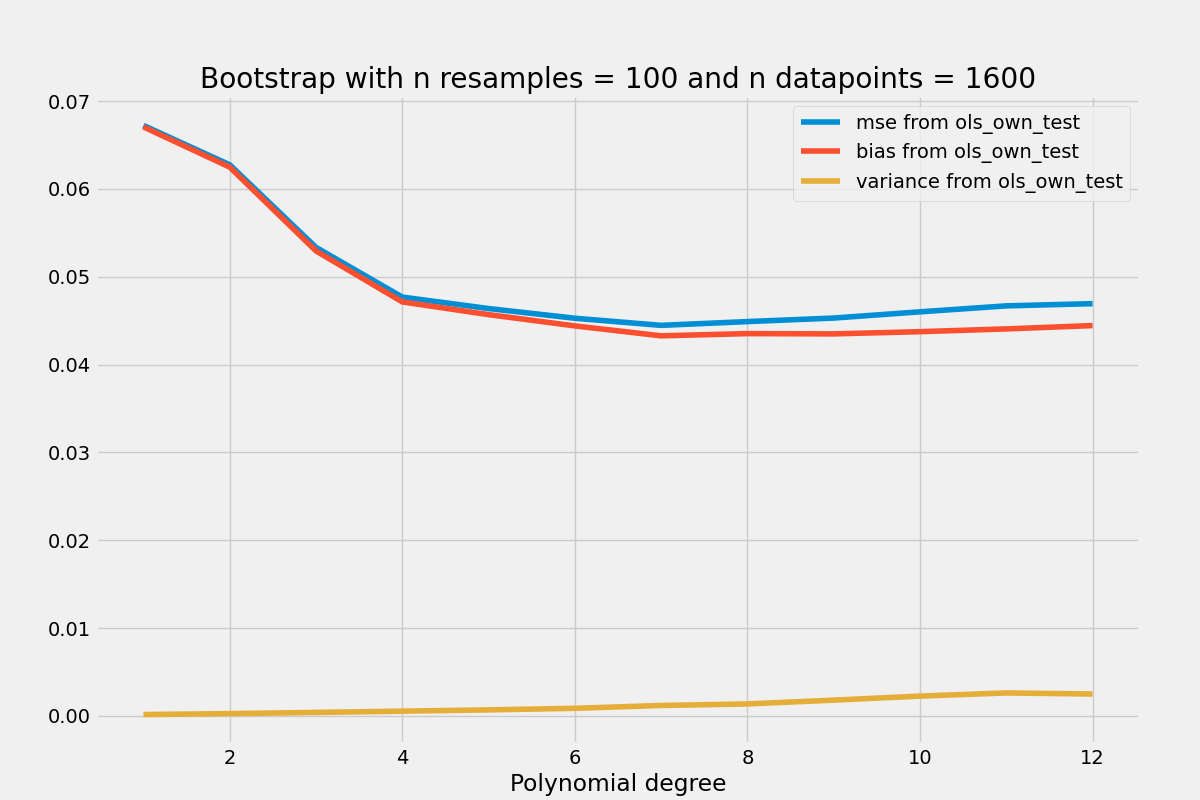
\includegraphics[width=0.8\textwidth]{Figures/c_bootstrap_ols_n_data_1600.png}
%\end{figure}

% XXX: Is this expected behaviour?
\begin{figure}[H]
    \centering
    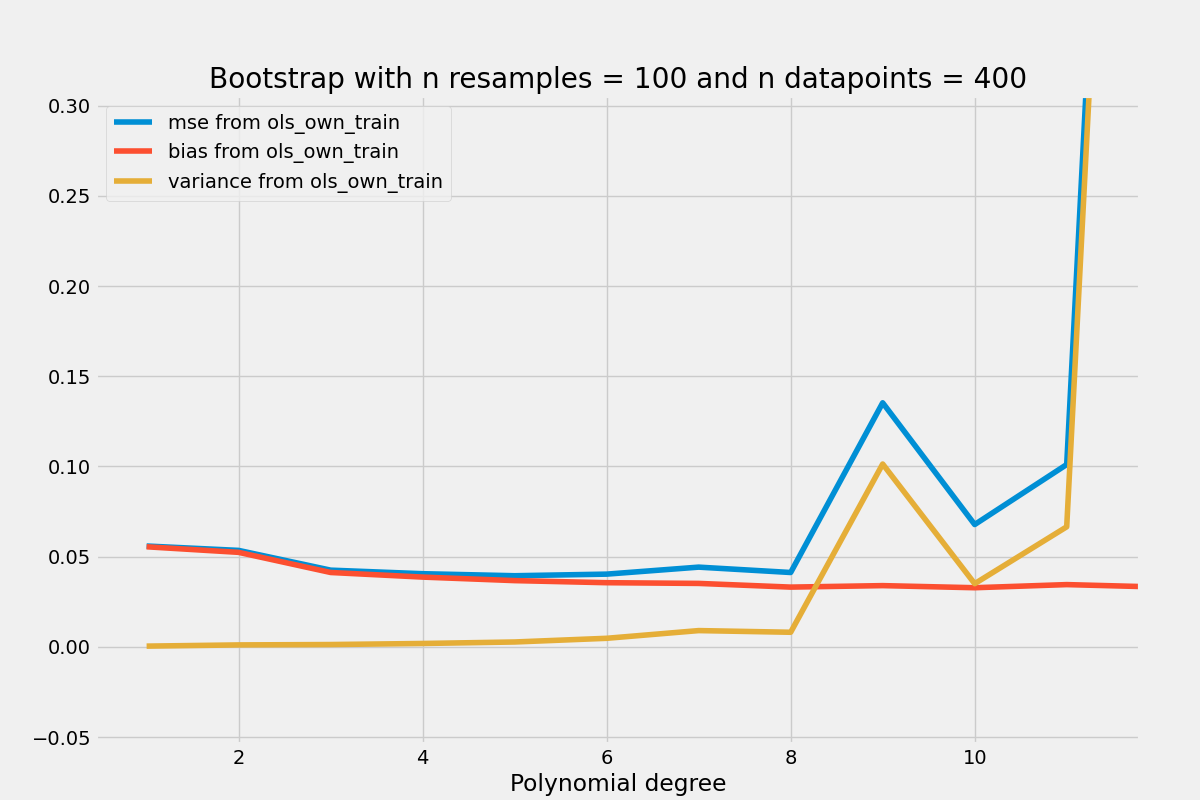
\includegraphics[width=0.8\textwidth]{Figures/c_bootstrap_ols_n_data_400_train_data.png}
    \caption{Bootstrap with 100 resamples for the OLS method on the Franke function on the training set with 400 datapoints.}
    \label{fig:bootstrap_ols_franke_train}
\end{figure}

To check the speculation of overfitting on the lower number of datapoints we look at figure \ref{fig:bootstrap_ols_franke_train} and we see here that the variance shoots off as the polynomial degree gets to 12. 

%%%%%%%%%%%%%%% Part d %%%%%%%%%%%%%%%
% Use k-fold and evaluate MEE on test data
% compare with bootstrap
% compare with sklearn

\begin{figure}[H]
    \centering
    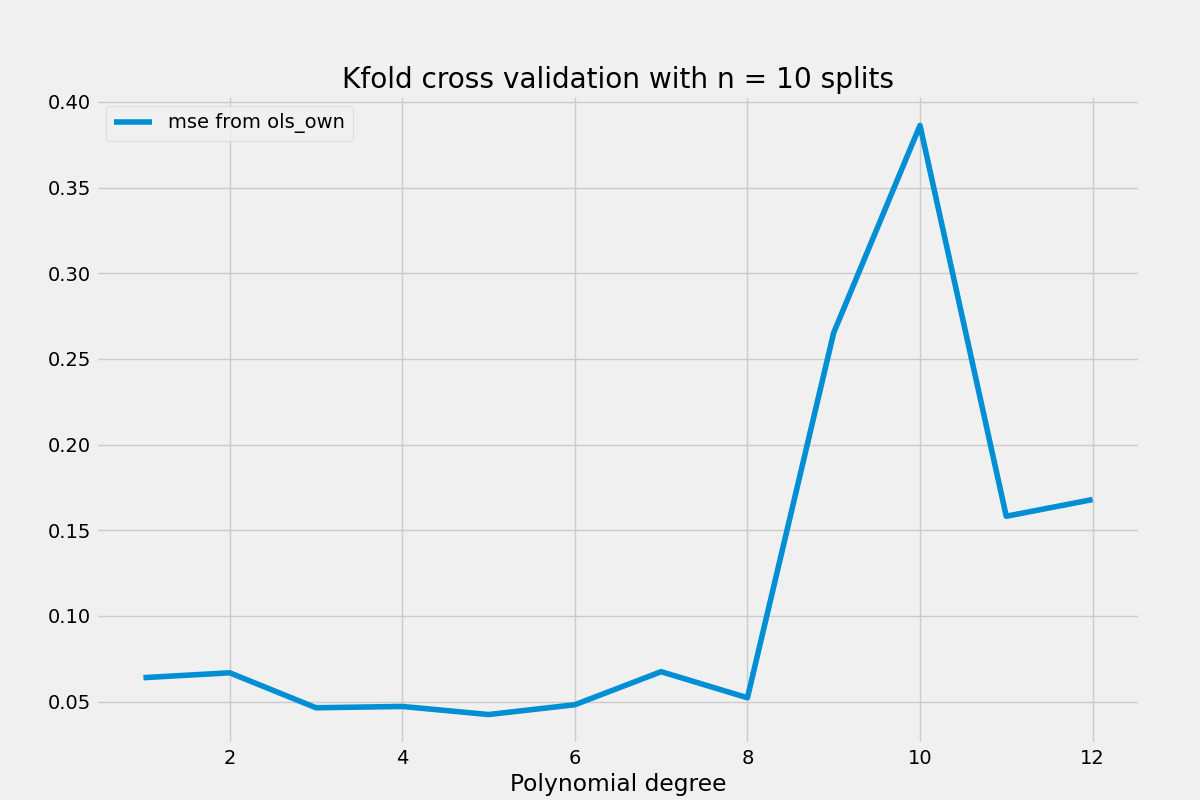
\includegraphics[width=0.8\textwidth]{Figures/d_kfold_ols_n_10.png}
    \caption{Mean squared error using cross-Validation with 10 splits on the Franke function.}
    \label{fig:kfold_ols_franke}
\end{figure}

In figure \ref{fig:kfold_ols_franke} we can see the MSE of Cross-validation with 10 spilts on the Franke function using OLS. This is on the test data. We see that polynomial degree over 8 produces weird results. This can be because of overfitting. 

%%%%%%%%%%%%%%% Part e %%%%%%%%%%%%%%%
% * bootstrap analysis for ridge as in part c
% * and cross validation as in part d 
% * Compare results to those obtained in part b-d
% * study bias variance trade off for different values of lambda 

The minimum MSE from Ridge regression was found for polynomial degree of 6 with
the hyper parameter, $\lambda = 0.001$. This is seen in figure \ref{fig:ridge_blabla}. Here we are to low in polynomial degree to see the typical bias-variance pattern.

\begin{figure}[H]
    \centering
    \caption{Ridge resgression. Franke function.}
    \label{fig:ridge_blabla}
    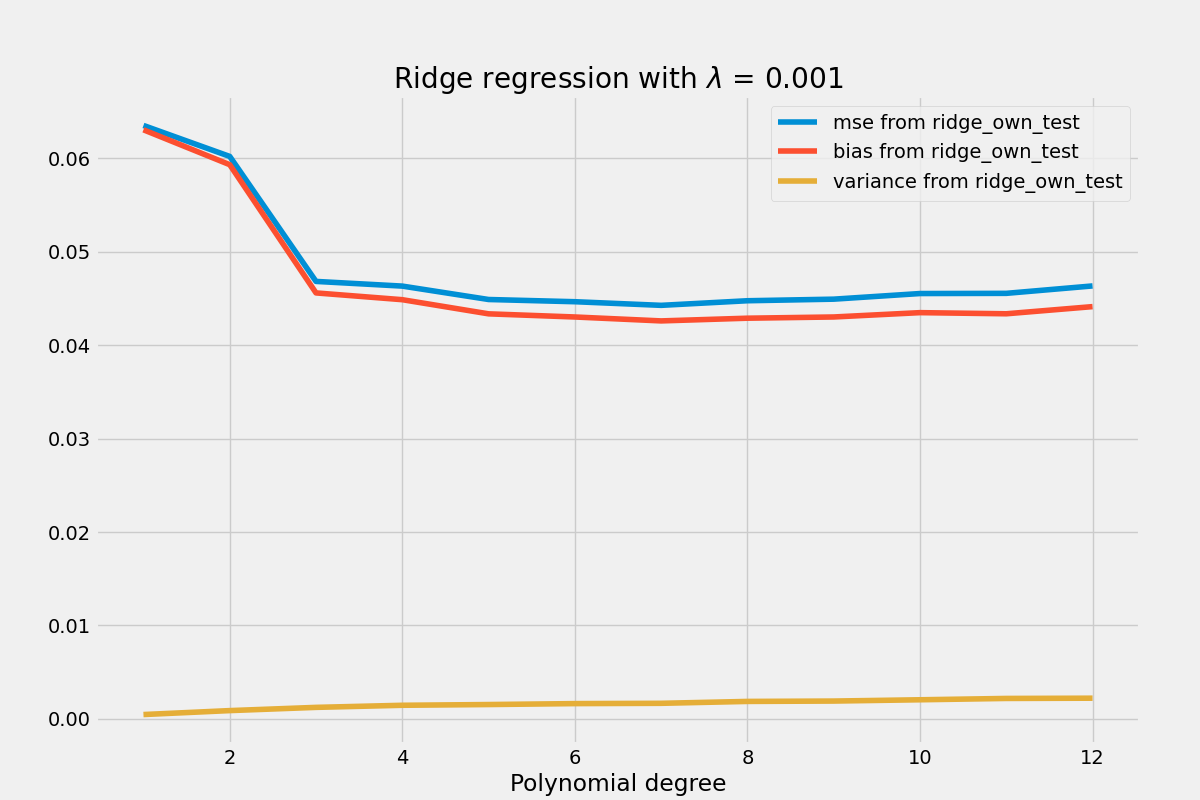
\includegraphics[width=0.8\textwidth]{Figures/e_ridge_bias_variance_lamb_0_001.png}
\end{figure}


\begin{figure}[H]
    \centering
    \caption{ridge bootstrap}  
    \label{fig:e_ridge} 
    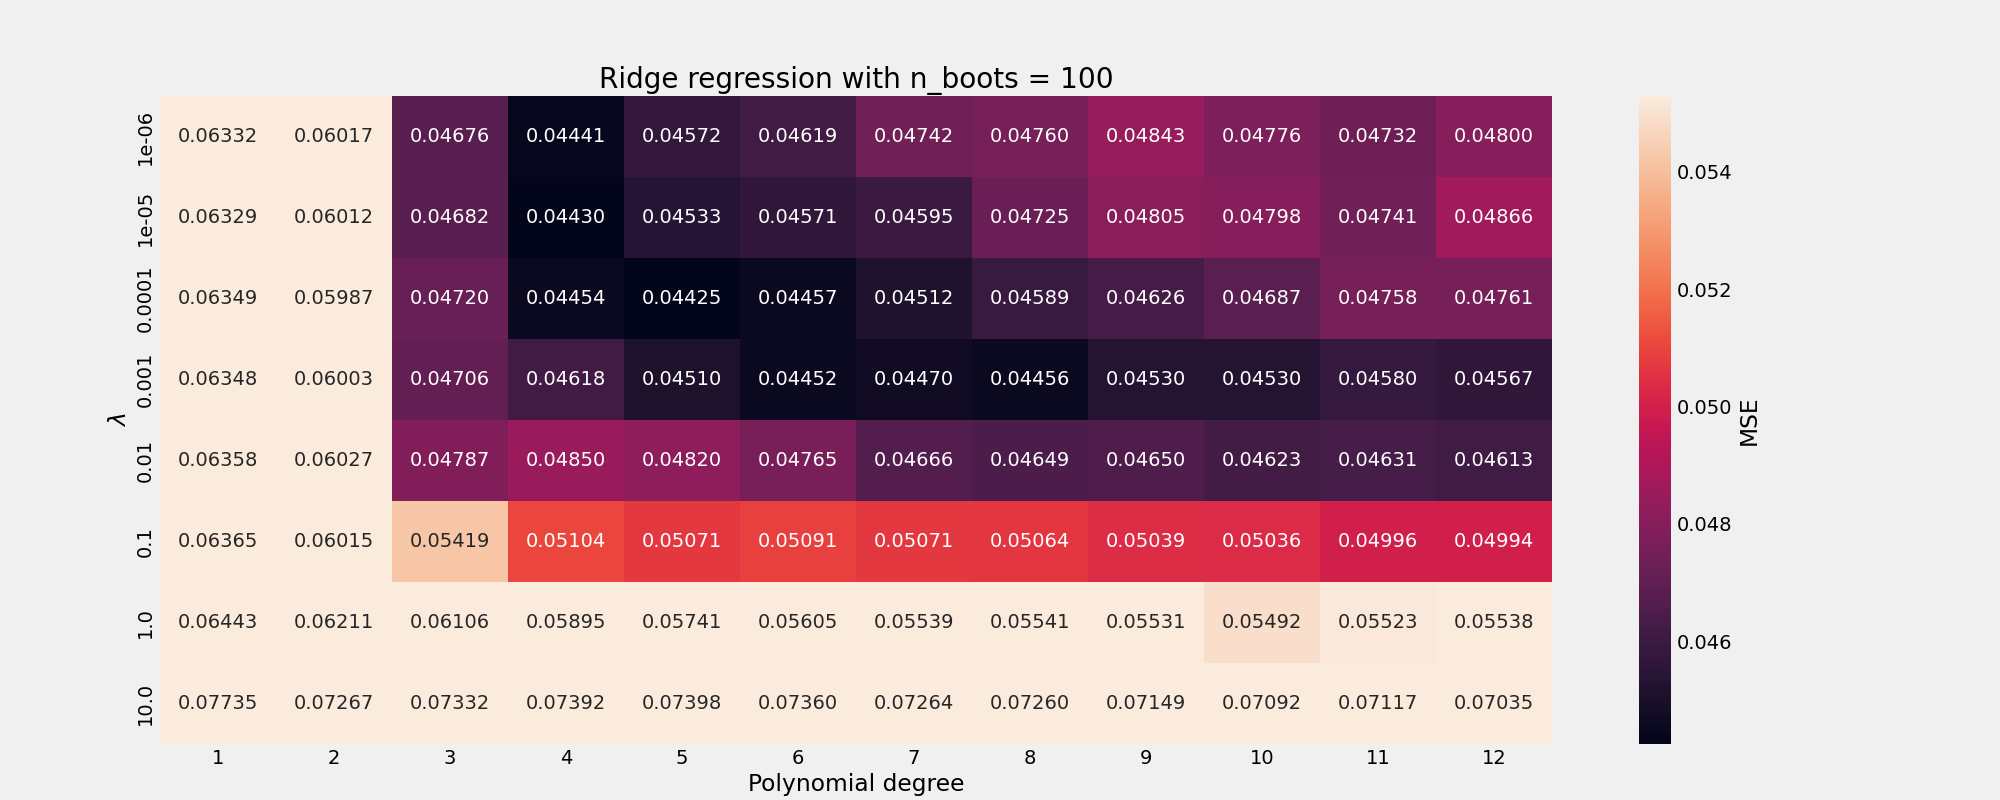
\includegraphics[width=1\textwidth]{Figures/e_ridge_n_boots_100.png}
\end{figure}

\begin{figure}[H]
    \centering
    \caption{ridge cv}
    \label{fig:e_ridge_kfold}
    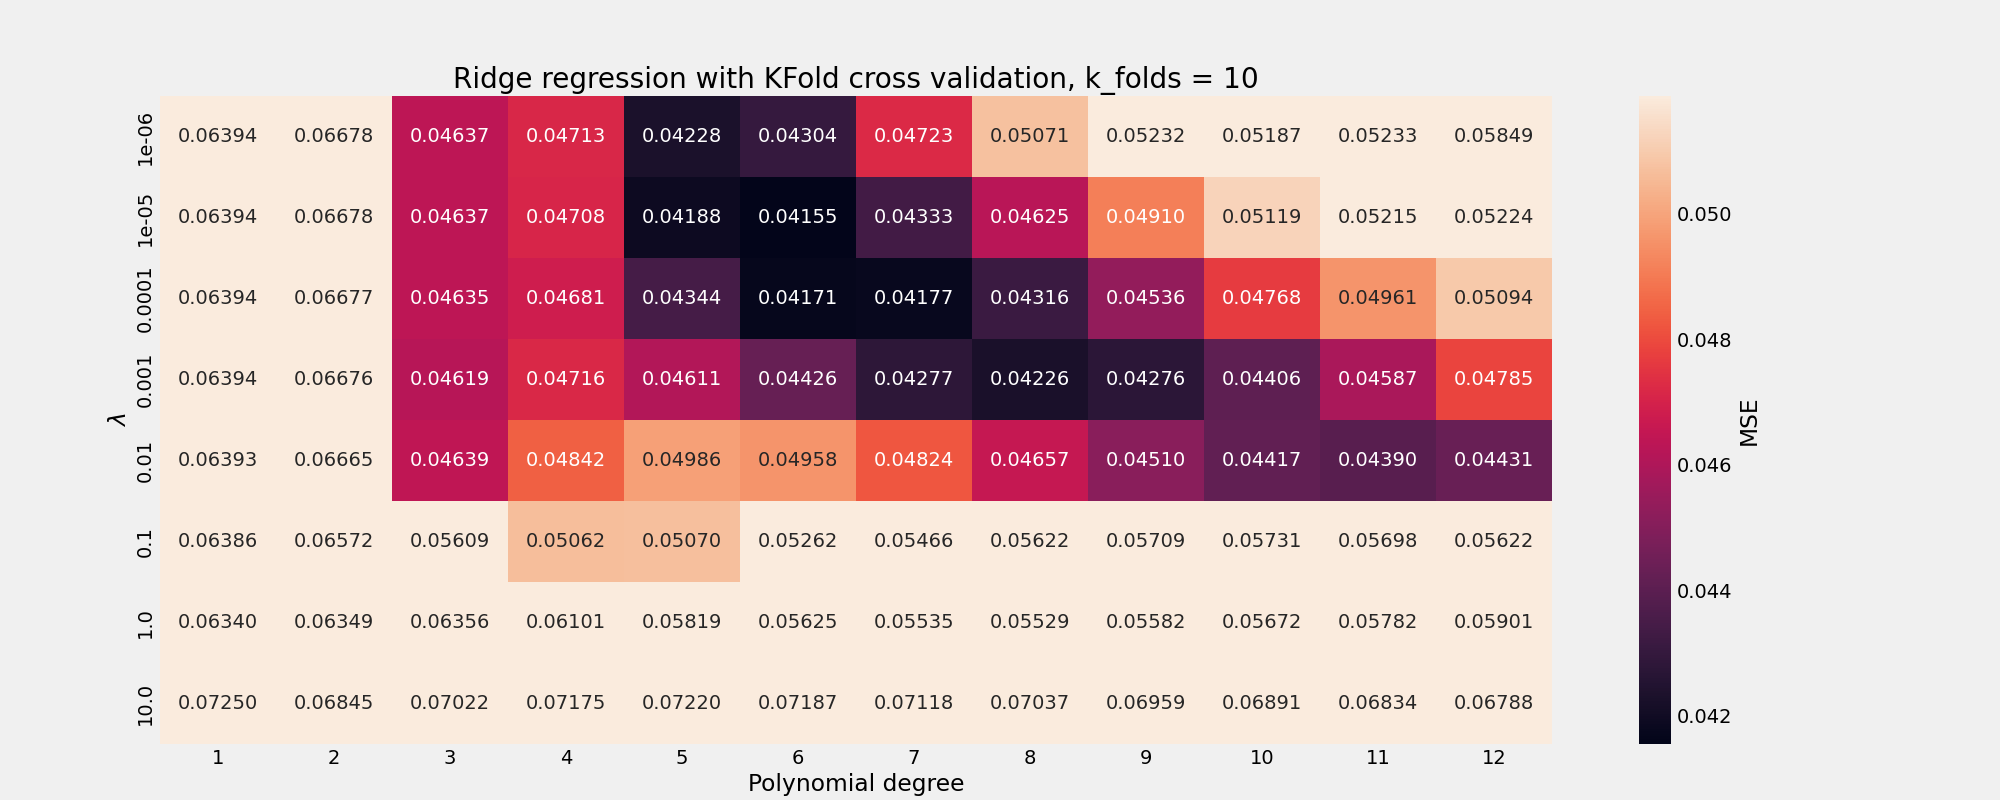
\includegraphics[width=0.8\textwidth]{Figures/e_ridge_kfold_n_10.png}
\end{figure}

Now we want to find the optimal $\lambda$ parameter 


%%%%%%%%%%%%%%% Part f %%%%%%%%%%%%%%%
% * Lasso regression
% * give a critical discussion of mse, ridge, lasso, in theory I discussed benefits of methods.
% * Which model fits the data best 
% * bootstrap bias variance analysis of lasso
% * MSE analysis with kfold


\begin{figure}[H]
    \centering
    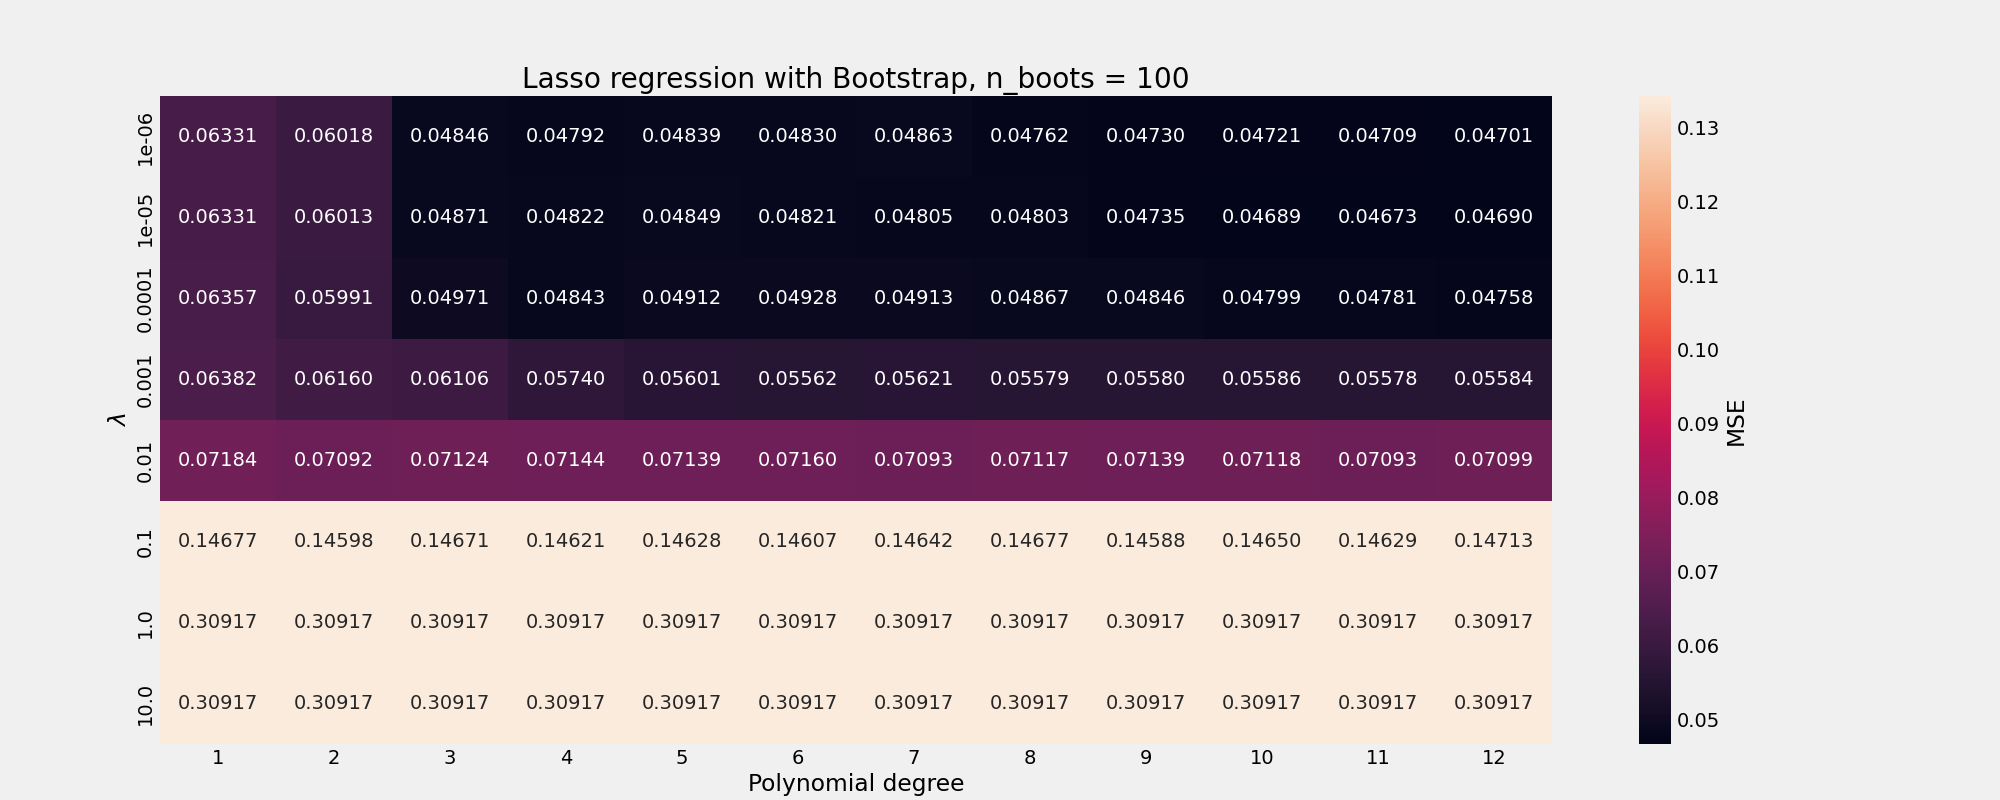
\includegraphics[width=0.8\textwidth]{Figures/f_lasso_bootstrap_n_100.png}
\end{figure}

\begin{figure}[H]
    \centering
    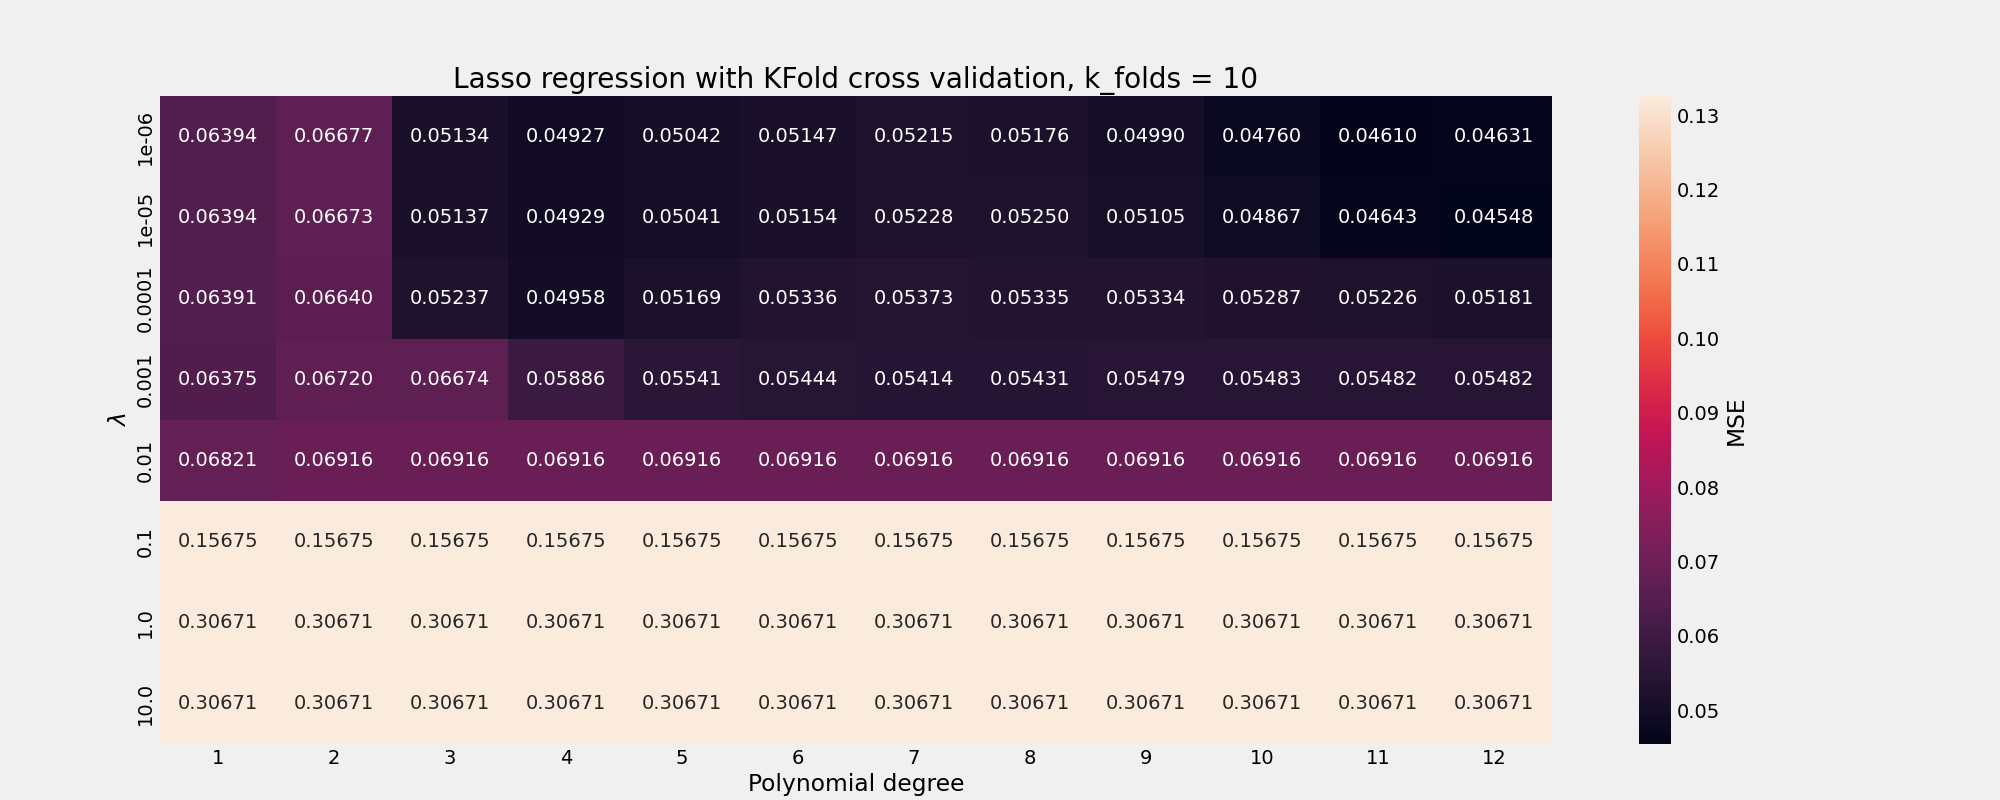
\includegraphics[width=0.8\textwidth]{Figures/f_lasso_kfold_n_10.png}
\end{figure}



% TODO: comparison of MSE for all methods
 
 %Maybe split results into two parts, Franke and Terrain data

%According to red line in report we want:
%On Franke-Function
%Subplot of MSE and R^2, test and training data, for OLS
%Subplot of MSE and R^2, test and training data, for Lasso
%Subplot of MSE and R^2, test and training data, for Ridge
%Comparrison of Regression methods
%Beta plot, but how to do this nicely, to show how beta values get large when polynomial degree increases.
%Resampling: bias-variance plot of bootstrap and cross-validation
%Study lambda dependence (correlation plot)

%On Terrain-data
%Subplot of MSE and R^2, test and training data, for OLS
%Subplot of MSE and R^2, test and training data, for Lasso
%Subplot of MSE and R^2, test and training data, for Ridge
%Comparrison of Regression methods
%Resampling: bias-variance plot of bootstrap and cross-validation
%Study lambda dependence (correlation plot)

%For critical discussion of centering/scaling, from lecture notes: "If our predictors represent different scales, then it is important to standardize the design matrix  by subtracting the mean of each column from the corresponding column and dividing the column with its standard deviation."




%%%%%%%%%%%%%%%%%%%%%%%%%%%%%%%%%%%%%%%%%%%%%
\subsection{Terrain data}
\begin{figure}[H]
    \centering
    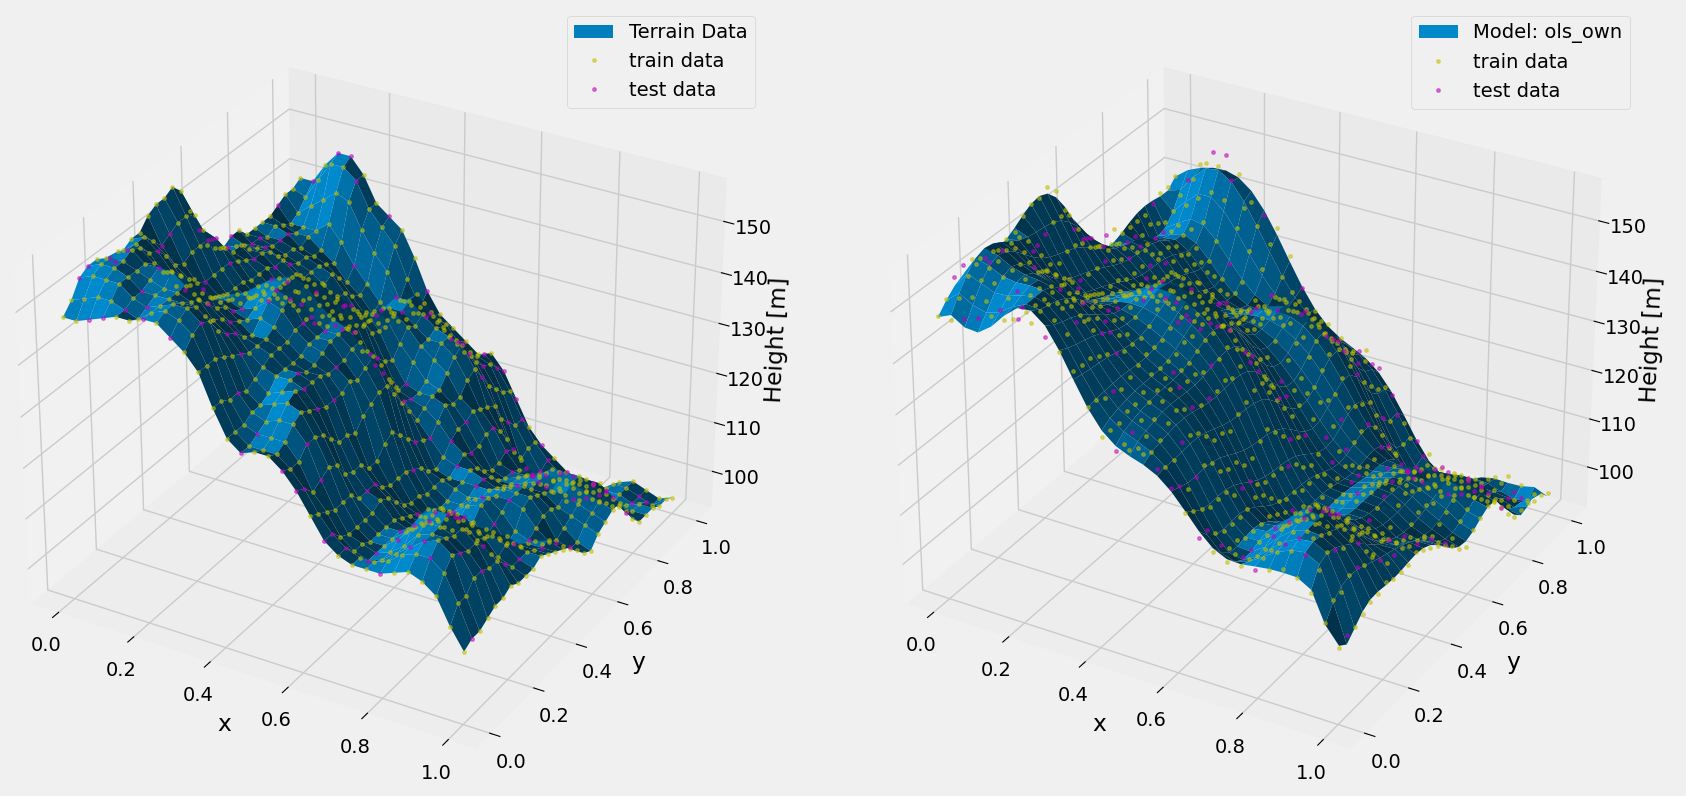
\includegraphics[width=0.8\textwidth]{Figures/terrain_data_and_model_ols_best.png}
    \caption{The left figure shows the surface of our sliced terrain data. Our
    train and test-data are represented by yellow and purple dots respectively.
Hight above sea level in meters is plotted on the z axis. The x- and y-axis is
takes values in intervall [0, 1]. This interval scales to 30m in real
coordinates. The left figure shows our best fit model obtained with OLS for
polynomial degree 18. Again the training- and test-data is plotted as in the
left figure.}  
\end{figure}

\begin{figure}[H]
    \centering
    \begin{subfigure}[b]{0.49\textwidth}
        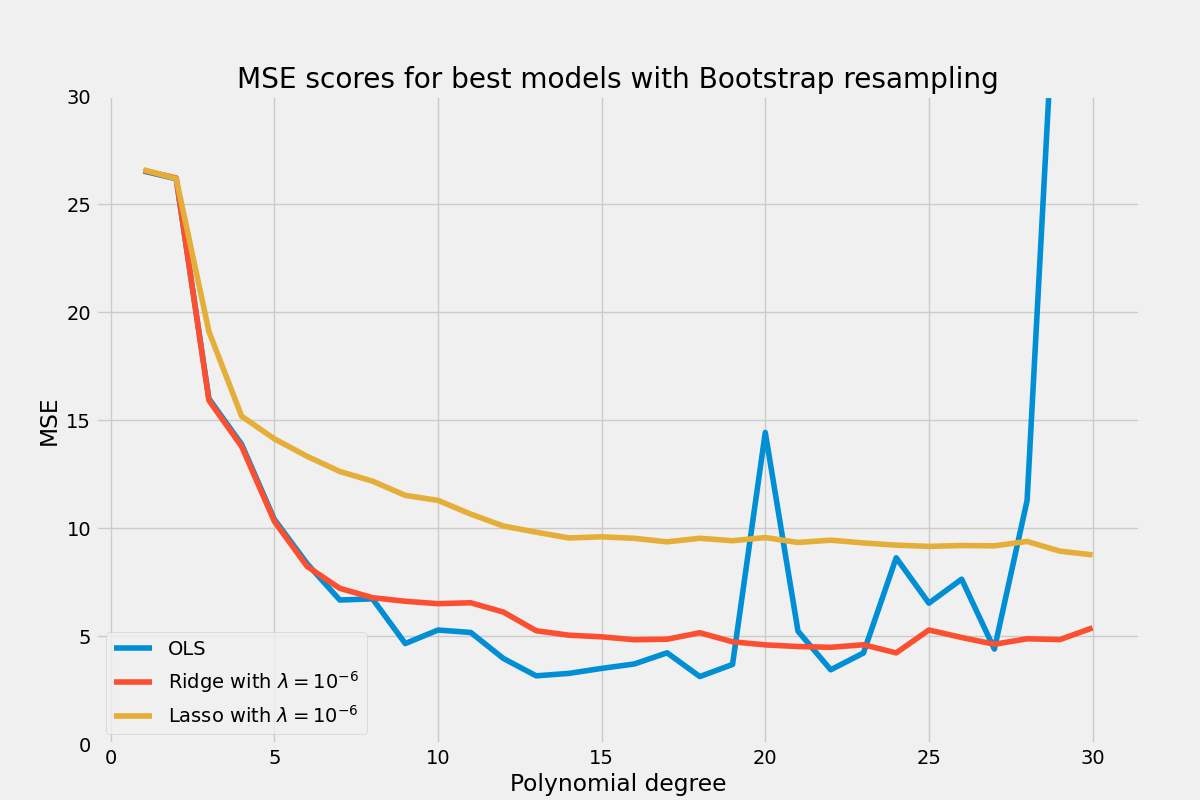
\includegraphics[width=\textwidth]{Figures/terrain_best_ols_ridge_lasso_boots.png}
        \caption{Mean of MSE scores calculated with bootstrap on the terrain data.\\ $n_{\text{boots}} =
        20$ re-samples was used. The mean MSE predicted on the test-data is plotted as
    function of polynomial degree for OLS-, Ridge- ($\lambda = 10^{6}$) and
Lasso-regression (\lambda = 10^{-6})   }  
    \end{subfigure}
    \begin{subfigure}[b]{0.49\textwidth}
        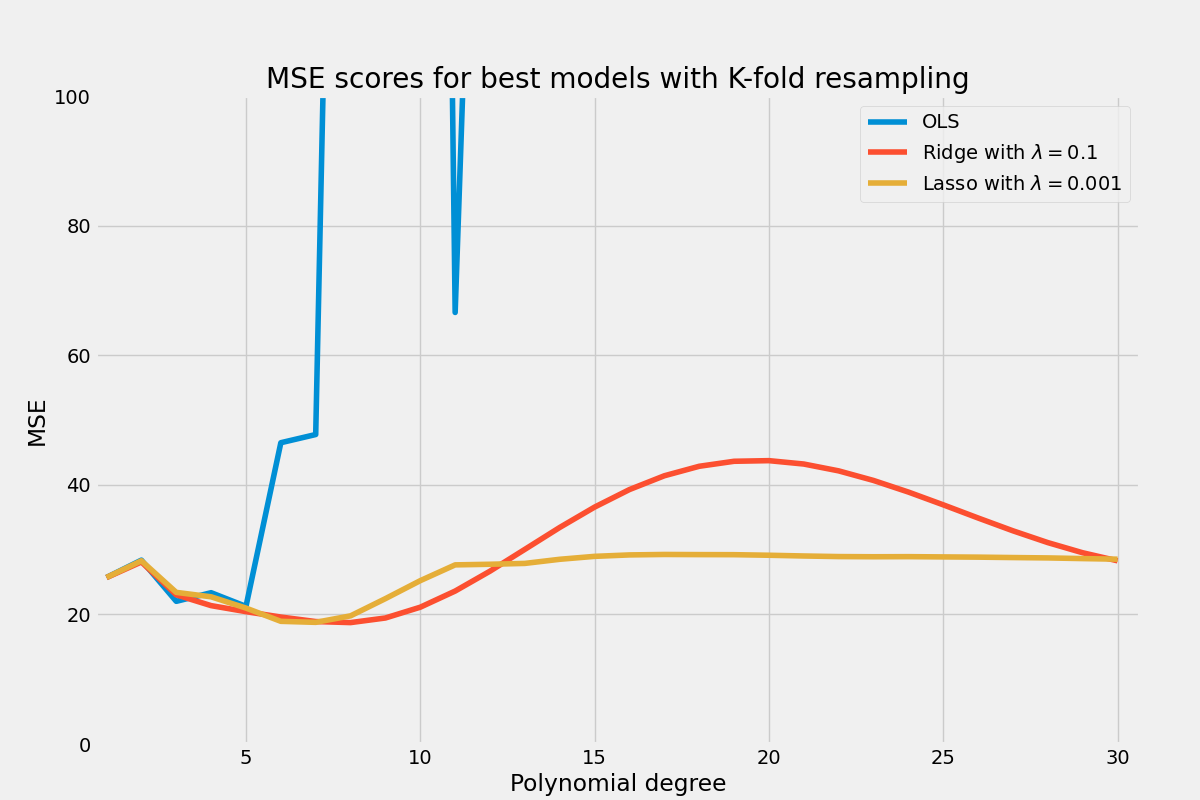
\includegraphics[width=\textwidth]{Figures/terrain_best_ols_ridge_lasso_kfold.png}
        \caption{Mean of MSE predicted on each test fold with use of the K-fold
        re-sampling technique. A total of ten folds was used. The MSE score is plotted as a function
    of polynomial degree for OLS-, Ridge- ($\lambda = 0.1$) and Lasso-regression
($\lambda = 10^{-4}$)}  
    \end{subfigure}
\end{figure}



\begin{figure}
\centering
\begin{subfigure}{0.49\textwidth}
    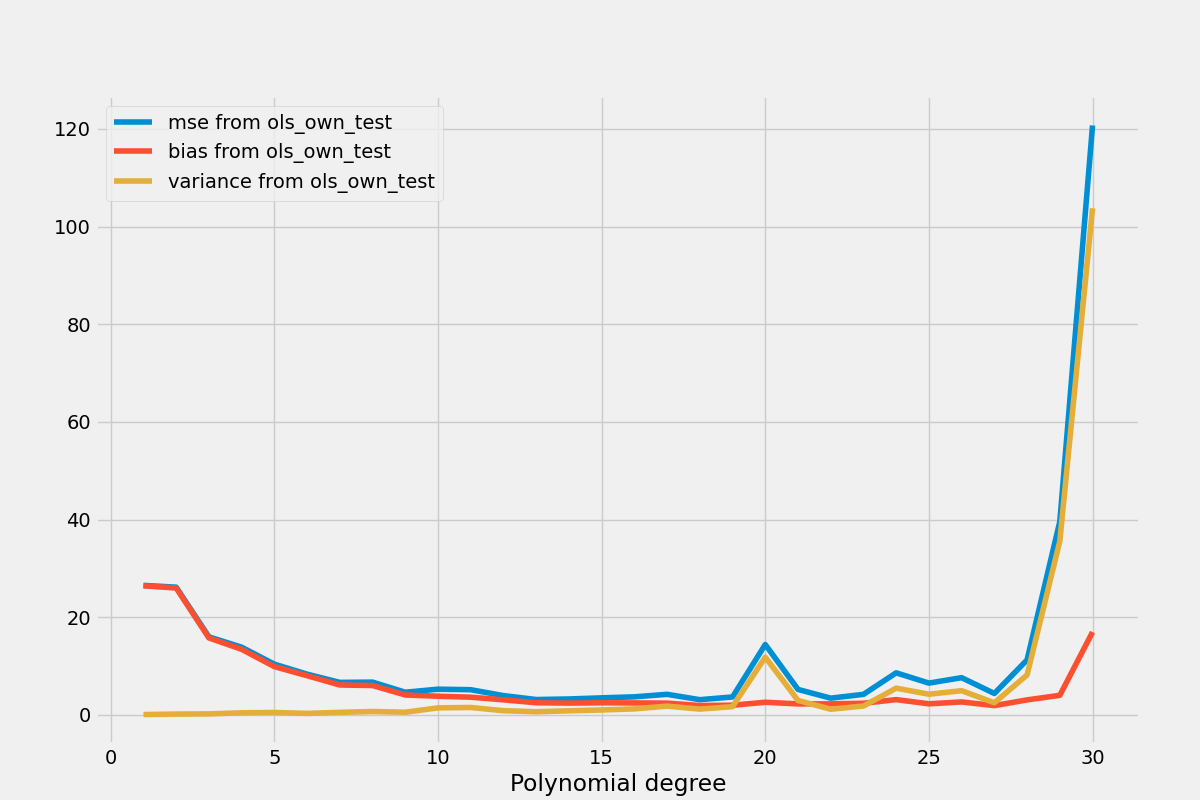
\includegraphics[width=\textwidth]{Figures/g_ols_bias_variance_boots_n_20.png}
    \caption{Bias, Variancse and MSE obtained with OLS and bootstrap re-sampling.
    20 re-samples was used to calculate the mean scores.}
    \label{fig:g_ols_bias_variance_boots}
\end{subfigure}
\hfill
\begin{subfigure}{0.49\textwidth}
    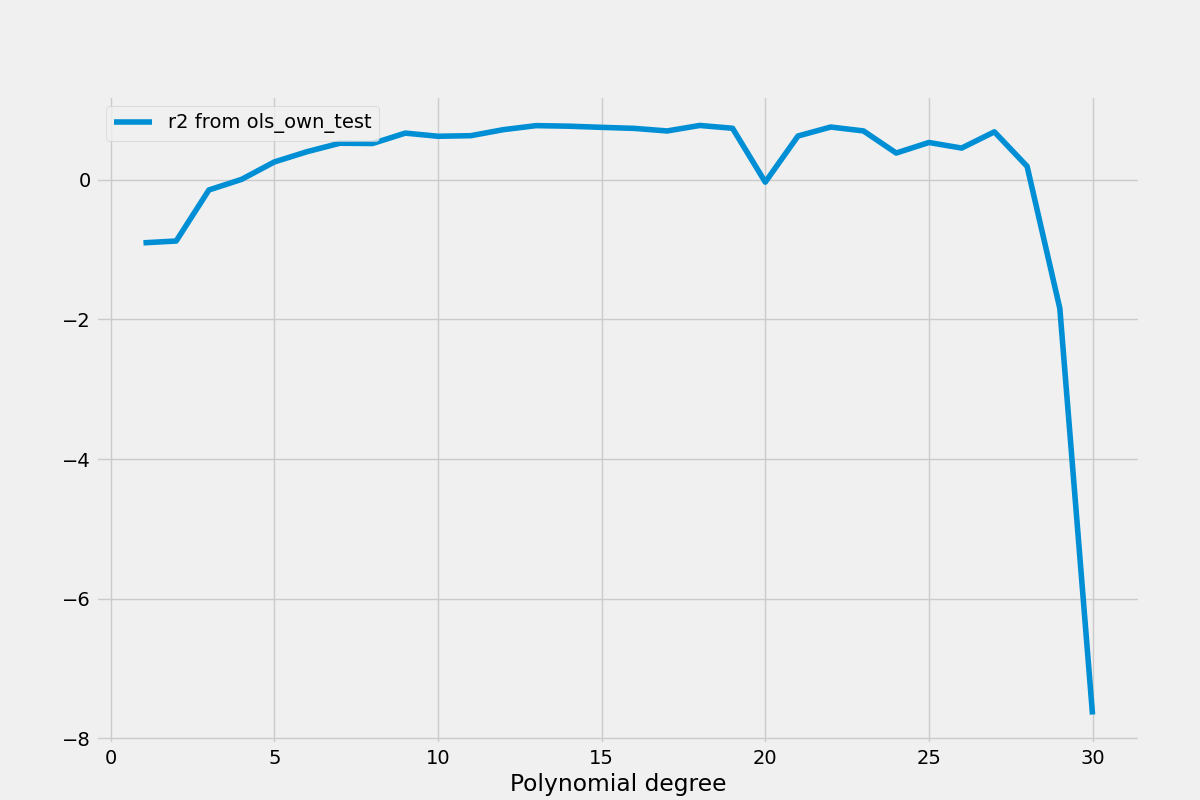
\includegraphics[width=\textwidth]{Figures/g_ols_r2_boots_n_20.png}
    \caption{R2 score obtained with OLS and bootstrap re-sampling.
    20 re-samples was used to calculate the mean R2 score.}
    \label{fig:g_ols_bias_variance_boots}
\end{subfigure}
\end{figure}


\begin{figure}[H]
    \centering
    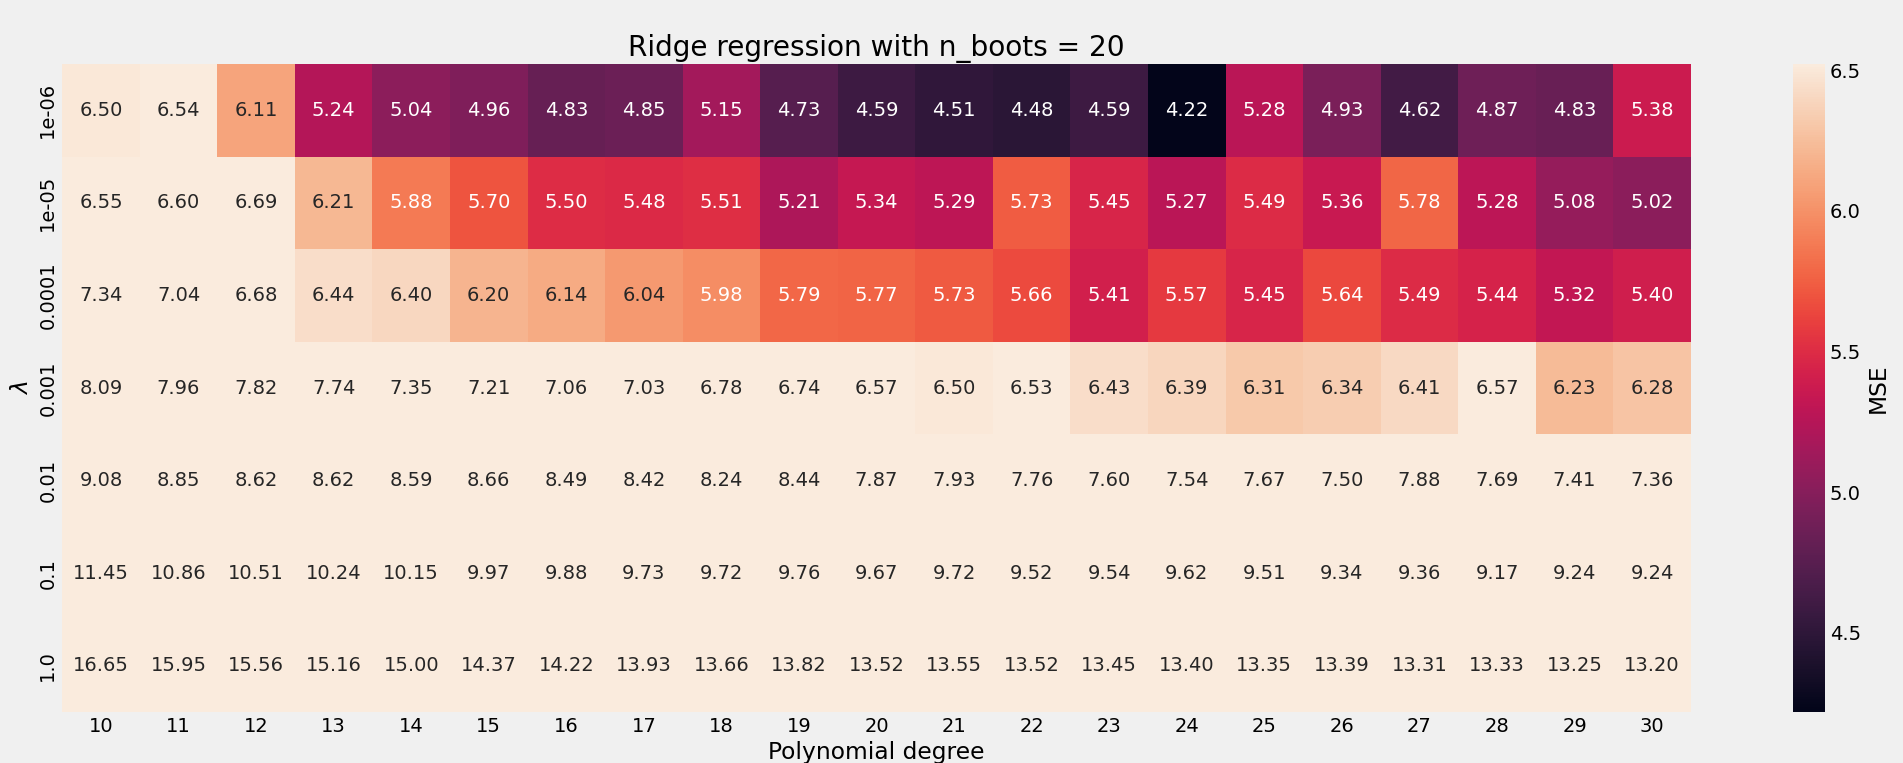
\includegraphics[width=\textwidth]{Figures/g_ridge_heatmap_boots_n_20.png}
    \caption{Heatmap of MSE scores obtained with Ridge regression and Bootstrap
    re-sampling, with 20 bootstrap re-sampling iterations.}  
    \label{fig:g_ridge_boost_heatmap}  
\end{figure}

\begin{figure}[H]
    \centering
    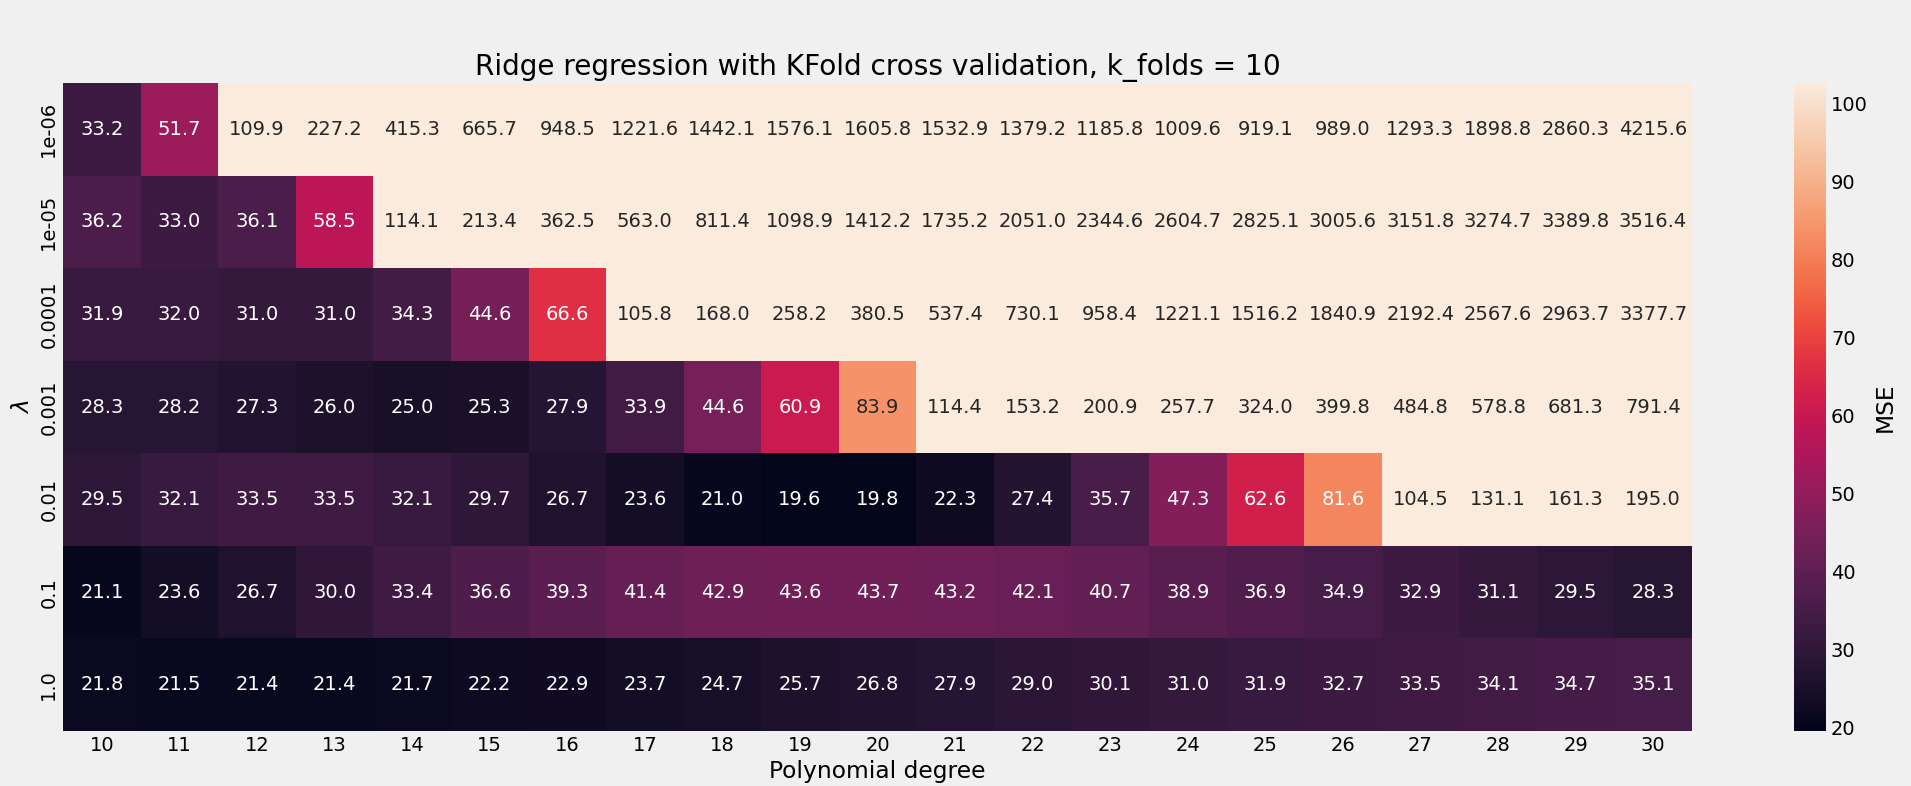
\includegraphics[width=\textwidth]{Figures/g_ridge_heatmap_kfold_n_10.png}
    \caption{Heatmap of MSE scores obtained with Ridge regression and K-fold
    re-sampling, with 10 splits.}  
    \label{fig:g_ridge_kfold_heatmap}  
\end{figure}

\begin{figure}[H]
    \centering
    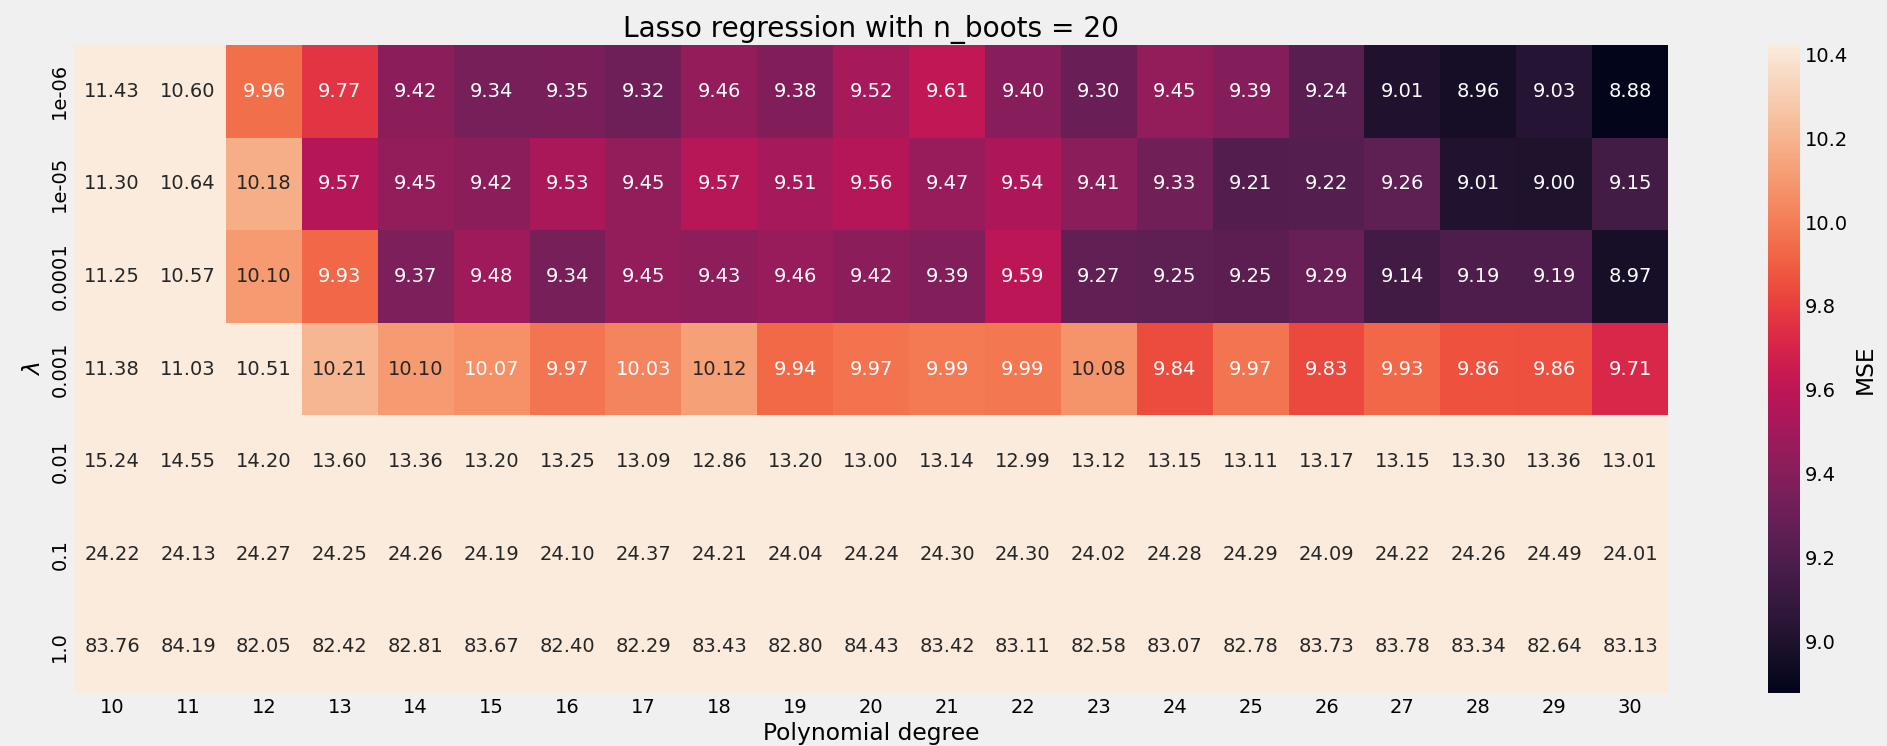
\includegraphics[width=\textwidth]{Figures/g_lasso_heatmap_boost_n_20.png}
    \caption{Heatmap of MSE scores obtained with lasso regression and Bootstrap
    re-sampling, with 20 re-samples.}  
    \label{fig:g_lasso_boots_heatmap}  
\end{figure}

\begin{figure}[H]
    \centering
    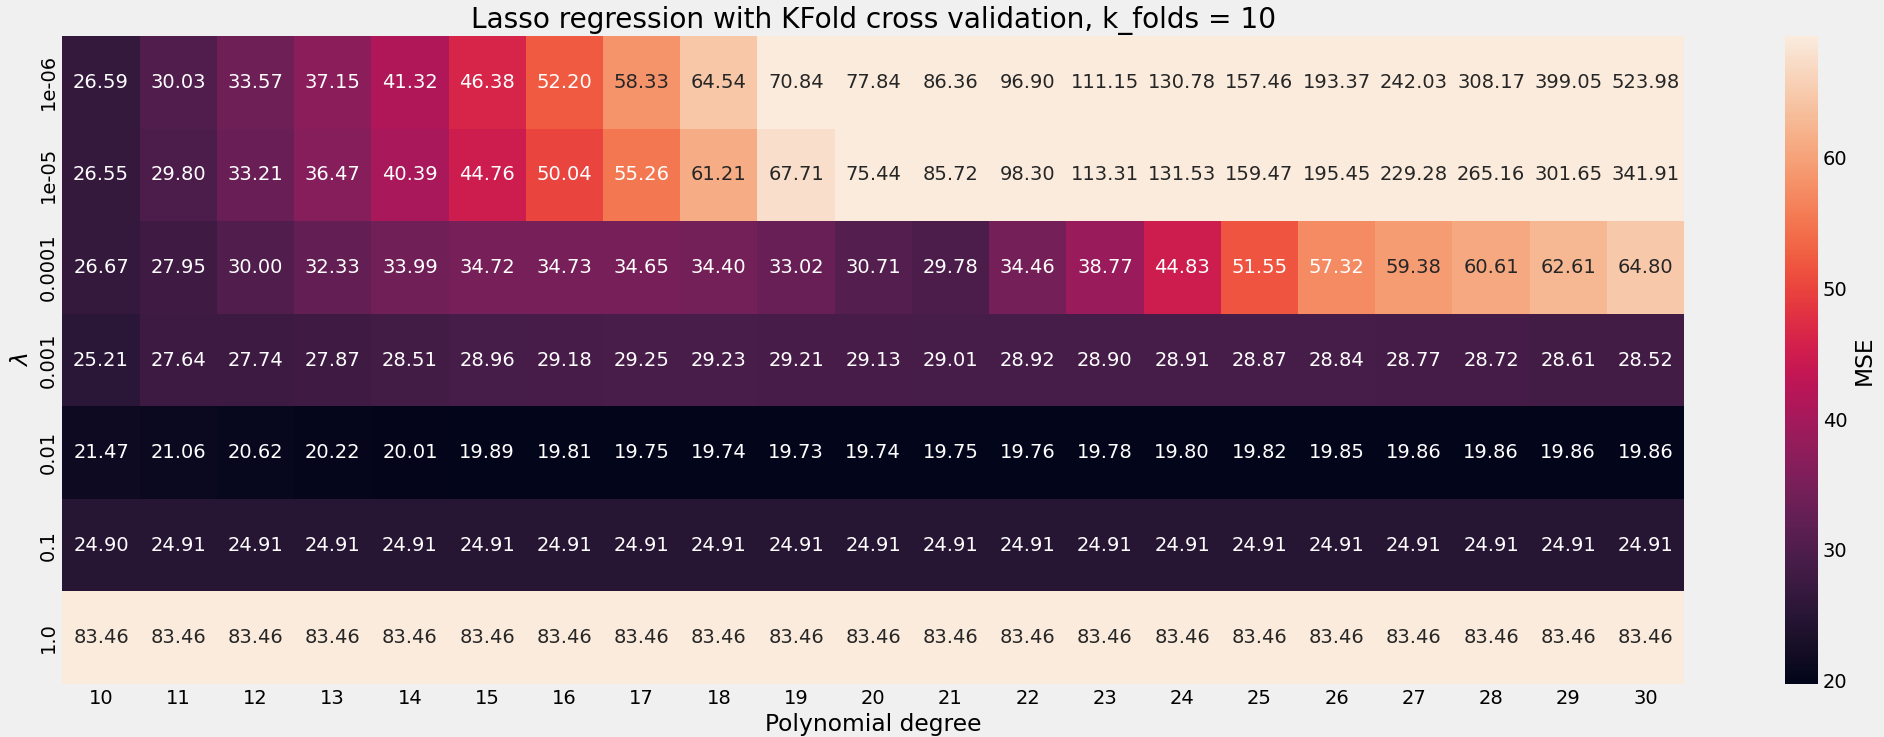
\includegraphics[width=\textwidth]{Figures/g_lasso_heatmap_kfold_n_10.png}
    \caption{Heatmap of MSE scores obtained with lasso regression and K-fold
    re-sampling, with 10 splits.}  
    \label{fig:g_lasso_boots_heatmap}  
\end{figure}



\begin{table}
    \centering
    \caption{Table of Best mean squared error (MSE) scores obtained with
        different re-sampling and regression
        methods. $\lambda $ is the best choice of regularization parameters for
        Ridge and Lasso regression. n refers to number of re-samples/splits used in
        Bootstrap and K-fold.}  
    \label{tab:terrain_mse_best} 
    \begin{tabular}{|c|c|c|c|c|}
        \hline
        Polynomial degree & $\lambda$ & Regression method & Re-sampling method & MSE \\
        \hline
                          18 &   &  OLS & Bootstrap (n=20) & 3.12\\
        \hline

                          24 & $10^{-6}$ &   Ridge & Bootstrap (n=20) & 4.22\\
        \hline

                          30 &  $10^{-6}$ & Lasso&  Bootstrap (n=20) & 8.88\\
        \hline

                          5 &  & OLS & K-fold (n=10)& 21.23\\
        \hline

                          8 &  0.1 & Ridge & K-fold (n=10)& 18.74\\ % XXX: new - forgot to inspect deg 0-10
                          % 19 &  0.01 & Ridge & K-fold (n=10)& 19.6  XXX: old
        \hline
                          7 & 0.001 &  Lasso & K-fold (n=10)& 18.77\\ % XXX: new
                          % 19 & 0.01 &  Lasso & K-fold (n=10)& 19.73\\ % XXX: old
        \hline
    \end{tabular} 
\end{table}




\begin{figure}[H]
    \centering
    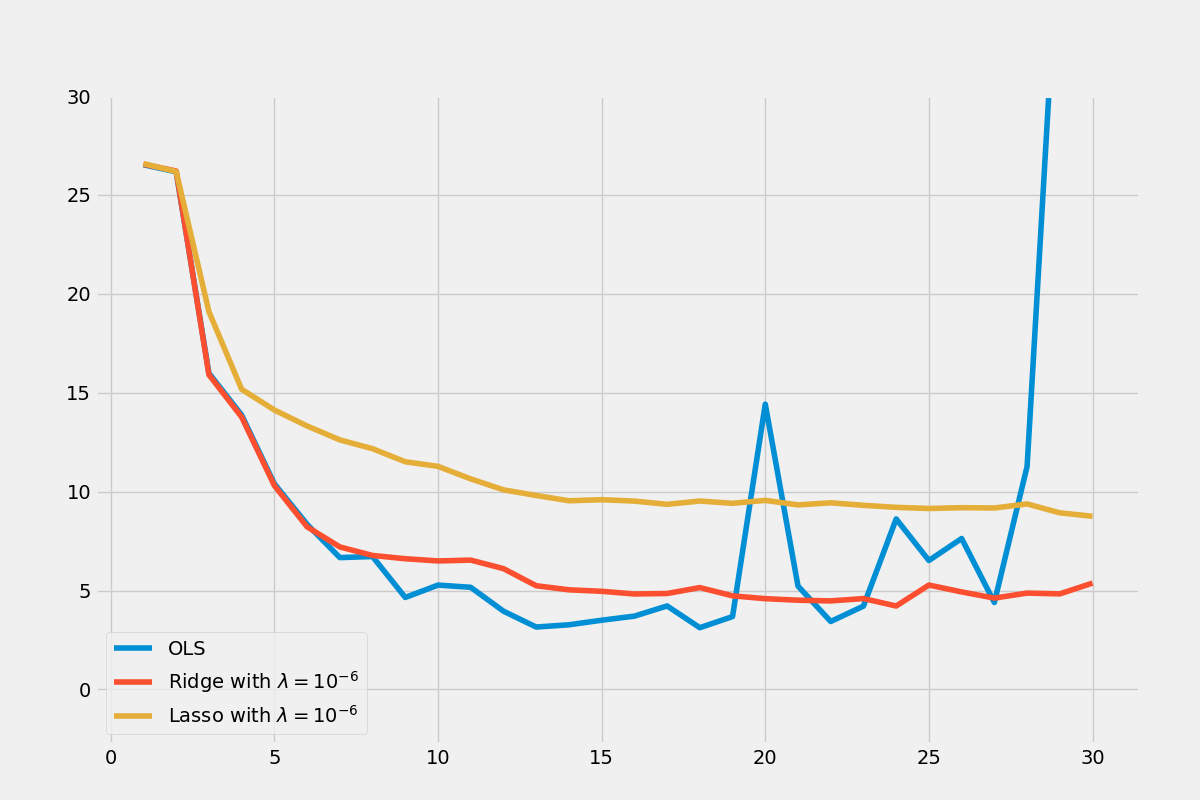
\includegraphics[width=0.8\textwidth]{Figures/g_ols_ridge_lasso_boots_n_20.png}
\end{figure}





